%----------------------------------------------------------------------------------------
%	CHAPTER 3
%----------------------------------------------------------------------------------------

%\chapterimage{boat.png}
\cleardoublepage
\chapterimage{chap_head.png}
\chapter{Transistors}

\section{Overview}\index{Overview}
In this section you'll learn about Light Emitting Diodes (LED) and how to turn it on using different methods.

\section{Component Introduction}\index{Component Introduction!Transistors}
In this chapter we will be using transistor to make electronic circuits. There are different types of transistors available but we will be using bipolar junction transistor (BJTs) only. BJTs are the most common transistor type used among the hobbyists and DIYers.

\subsection{BJT}
A transistor is a semiconductor device with 3 terminals or regions. The interface between each of the regions forms a p-n junction, it likes two diodes together. There are two types of BJTs -
NPN, when a p-type semiconductor is in-between two n-type.
PNP, when a n-type semiconductor is in-between two p-type.
Transistors are used to amplify or switch electronic signals and electrical power. Each of the terminals or regions are named - 
\begin{itemize}
    \item Collector: The largest semiconductor region of the transistor.
    \item Emitter: The second largest semiconductor region of the transistor.
    \item Base: Middle region of the transistor. This serves as a gatekeeper that determines the amount of current that can flow through emitter-collector regions.
\end{itemize}
\begin{figure}[!htp]
    \centering
    \begin{subfigure}[b]{0.4\textwidth}
        \centering
        \begin{circuitikz}[scale = 2]
            \draw
                (0,0) node [npn](npn1){}
                (npn1.E) node[right=1mm]{E}
                (npn1.C) node[right=1mm]{C}
                (npn1.B) node[left=1mm]{B};
        \end{circuitikz}
        \caption{NPN}
    \end{subfigure}
    \hfill
    \begin{subfigure}[b]{0.4\textwidth}
        \centering
        \begin{circuitikz}[scale = 2]
            \draw
                (0,0) node [pnp](pnp1){}
                (pnp1.E) node[right=1mm]{E}
                (pnp1.C) node[right=1mm]{C}
                (pnp1.B) node[left=1mm]{B};
        \end{circuitikz}
        \caption{PNP}
    \end{subfigure}
    \caption{Transistor Symbol}
    \label{fig:bjt_symbol}
\end{figure}

\subsubsection{Operation Modes for Transistor}
There are 4 modes in which a transistor works -
\begin{enumerate}
    \item \textbf{Cut-off}
    In cut-off mode no current flows through the transistor. The transistor acts like an open circuit.
    \item \textbf{Saturation}
    In saturation mode the transistor allows current to flow freely and acts like an short-circuit.
    \item \textbf{Active}
    In active mode the amount of current flowing through the collector-emitter region is proportional to the current flowing through base.
    \item \textbf{Reverse-Active}
    It is similar to active mode, but the direction of current is reversed. The transistors are not meant to operate in Reverse-Active mode.
\end{enumerate}
If we make sure that the transistor operates in only cut-off or saturation region, then it can act like a switch turning current flow ON or OFF by controlling the base voltage. In this guide most of the circuits will use transistor in Saturation \& cut-off mode.
\begin{figure}[!ht]
    \centering
    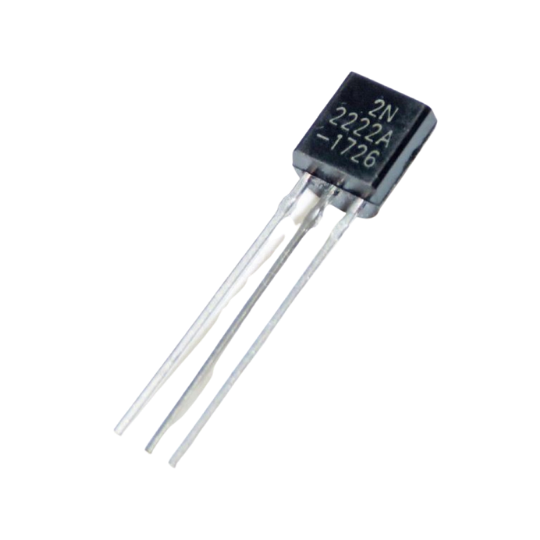
\includegraphics[width=0.4\textwidth]{Components/2n2222.png}
    \caption{Transistor}
    \label{fig:npn_code}
\end{figure}
In NPN transistor, the base voltage should be higher than the emitter voltage by threshold voltage $V_{th}$, defined in the data-sheet of the transistor. Generally it is near about \SI{0.7}{\volt}.

For PNP, the base voltage should be lower than the emitter voltage by $V_{th}$.
\begin{figure}[!htp]
    \centering
    \begin{subfigure}[b]{0.4\textwidth}
        \centering
        \begin{circuitikz}[scale = 2]
            \draw
                (0,0) node [npn](npn1){}
                (npn1.E) node[right=1mm](n1){E}
                (npn1.C) node[right=1mm](n2){C}
                (npn1.B) node[left=1mm](n3){B};
            \draw[-latex]
                (-1,0) -- (n3);
            \draw[-latex]
                (n2) -- (n1);
        \end{circuitikz}
        \caption{NPN}
    \end{subfigure}
    \hfill
    \begin{subfigure}[b]{0.4\textwidth}
        \centering
        \begin{circuitikz}[scale = 2]
            \draw
                (0,0) node [pnp](pnp1){}
                (pnp1.E) node[right=1mm](n1){E}
                (pnp1.C) node[right=1mm](n2){C}
                (pnp1.B) node[left=1mm](n3){B};
            \draw[-latex]
                (n3) -- (-1,0);
            \draw[-latex]
                (n1) -- (n2);
        \end{circuitikz}
        \caption{PNP}
    \end{subfigure}
    \caption{Direction of Conventional current in BJTs}
    \label{fig:bjt_current}
\end{figure}

For both the transistors, $I_E = I_C + I_B$

\subsection{Capacitor}
Capacitor is a pretty simple electronic device. It consists of two conductive plates separated by an insulated medium called dielectric. Capacitors when powered are able to store energy in the form of electric field between the two plates. With different types of dielectric, there are different types of capacitors and have different qualities and uses. Capacitors can be polarized when dielectric used is polarized and favours electric field in one direction. 
\begin{figure}[!htp]
    \centering
    \begin{subfigure}[b]{0.4\textwidth}
        \centering
        \begin{circuitikz}[scale = 2]
            \draw
                (0,0) to[capacitor] (0,1);
        \end{circuitikz}
        \caption{Non Polarized}
    \end{subfigure}
    \hfill
    \begin{subfigure}[b]{0.4\textwidth}
        \centering
        \begin{circuitikz}[scale = 2]
            \draw
                (0,0) to[curved capacitor] (0,1);
        \end{circuitikz}
        \caption{Polarized}
    \end{subfigure}
    \caption{Capacitor Symbol}
    \label{fig:cap_symbol}
\end{figure}
The value of capacitor is measured in Farads (F), and one farad is a very big value. \emph{The capacitance of earth is \SI{710}{\micro\farad}}.
\begin{figure}[!ht]
    \centering
    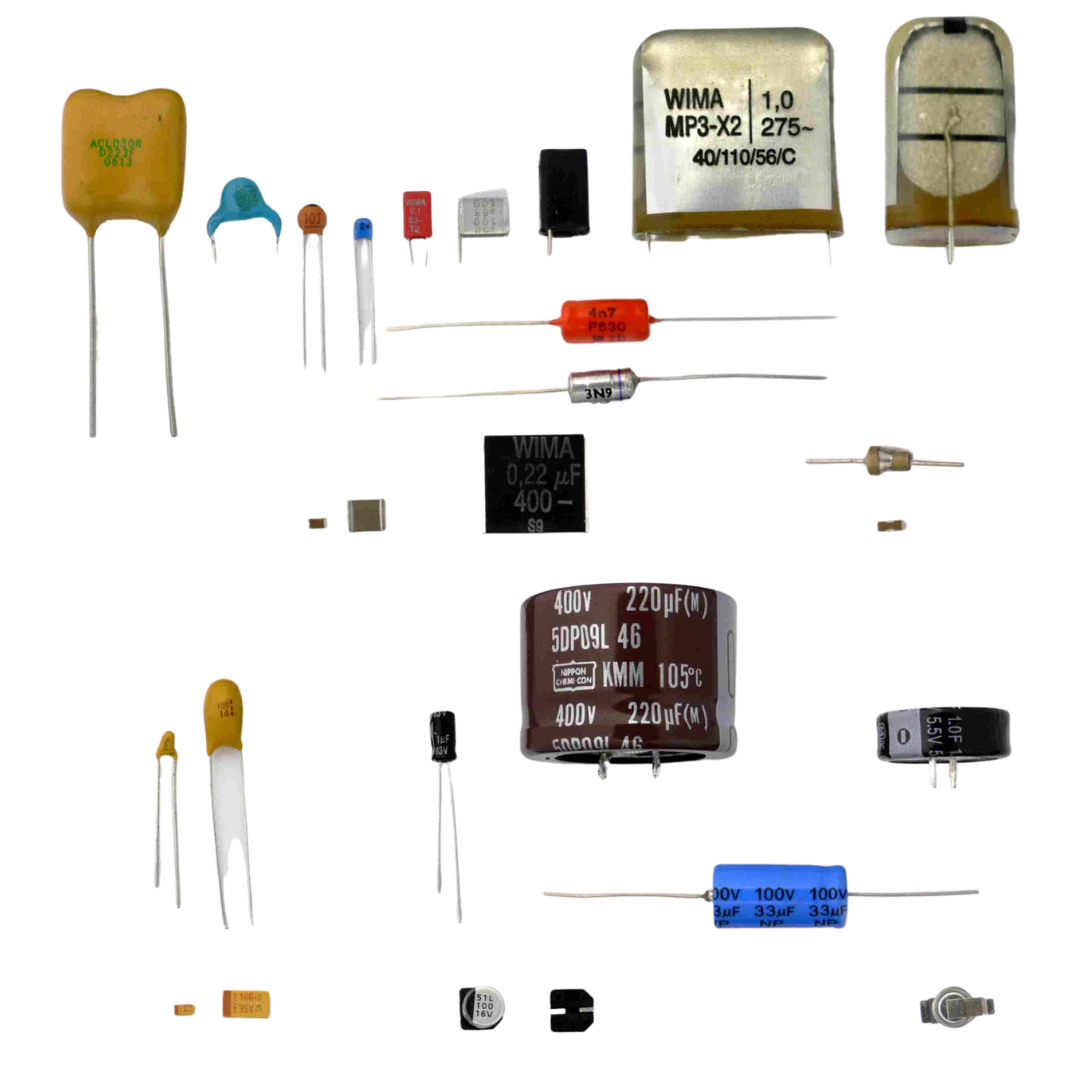
\includegraphics[width=0.6\textwidth]{Components/capacitors.png}
    \caption{Different types of Capacitors}
    \label{fig:cap_code}
\end{figure}
Capacitors or Caps are used in many ways and can be found in almost every electronic circuits.
On Polar capacitors the exact values in written on the body, for ceramic capacitor the values is written with 2 significant digits and 1 multiplier, for example capacitance of a ceramic capacitor with 105 written on it is, \num{10e4}\si{\pico\farad} = \num{e5}$\times$\num{e-12}\si{\farad} = \num{e-7}\si{\farad} = \SI{0.1}{\micro\farad}

\subsection{LDR}
Light Dependent Resistor(LDR) or photocell or photo-resistor is a semiconductor device which exhibits a very special property, it acts like a resistor but the value of resistance depends on the amount of light falling on it.
\begin{figure}[!ht]
    \centering
    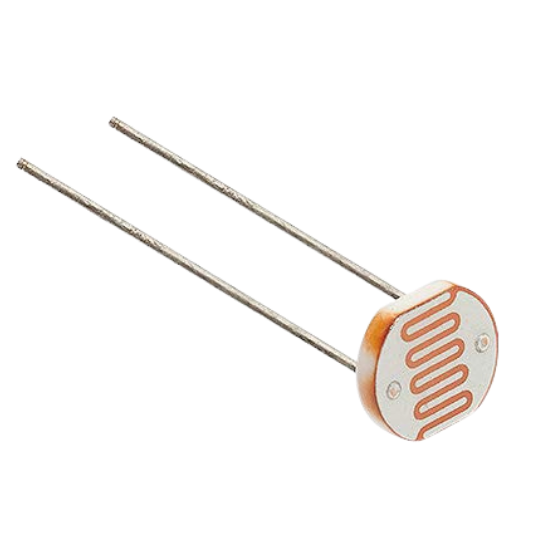
\includegraphics[width=0.4\textwidth]{Components/ldr.png}
    \caption{LDR}
    \label{fig:ldr_code}
\end{figure}
In bright light, the LDR resistance will be in the range of 0.01-10\si{\kilo\ohm} and in darkness it's resistance will be in the range of 100-1000\si{\kilo\ohm}.
\begin{figure}[!htp]
    \centering
    \begin{circuitikz}[scale = 2]
        \draw (0,0) to[sR] (1,0);
    \end{circuitikz}
    \caption{LDR Symbol}
    \label{fig:ldr_symbol}
\end{figure}

\subsection{RGB LED}
RGB LED is a combination of all three LEDs (RED, GREEN, BLUE) in one single package. You can produce different colors using RGB LEDs by configuring the intensity of each LED.
\begin{figure}[!ht]
    \centering
    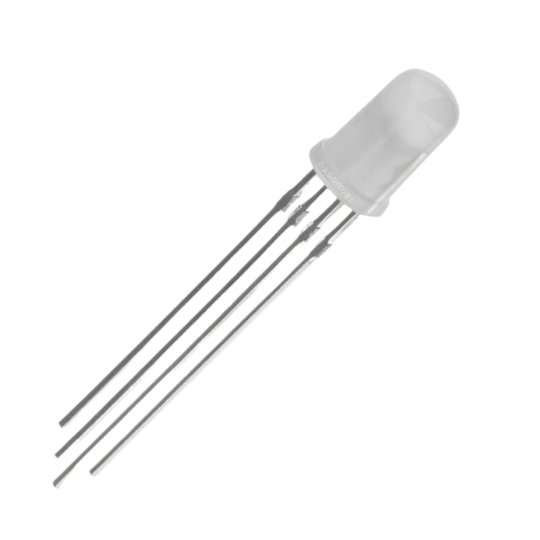
\includegraphics[width=0.4\textwidth]{Components/rgb-led.png}
    \caption{RGB LED}
    \label{fig:rgb_code}
\end{figure}
There are two kinds of RGB LED, one shares the cathode pin and the other shares the anode pin.
\begin{figure}[!htp]
    \centering
    \begin{subfigure}[b]{0.4\textwidth}
        \centering
        \begin{circuitikz}[scale = 2]
        \draw (0,0) to[short, *-] (0,0) -- ++(0,-0.5);
        \draw (0,0) to[full led, invert, color=green] (0,1);
        \draw (0,0) -- (0.5,0) to[full led, invert, color=red] (0.5,1);
        \draw (0,0) -- (-0.5,0) to[full led, invert, color=blue] (-0.5,1);
        \end{circuitikz}
        \caption{Common Anode}
    \end{subfigure}
    \hfill
    \begin{subfigure}[b]{0.4\textwidth}
        \centering
        \begin{circuitikz}[scale = 2]
        \draw (0,0) to[short, *-] (0,0) -- ++(0,-0.5);
        \draw (0,0) to[full led, color=green] (0,1);
        \draw (0,0) -- (0.5,0) to[full led, color=red] (0.5,1);
        \draw (0,0) -- (-0.5,0) to[full led, color=blue] (-0.5,1);
        \end{circuitikz}
        \caption{Common Cathode}
    \end{subfigure}
    \caption{RGB LED Symbol}
    \label{fig:rgb_symbol}
\end{figure}

\clearpage

\section{Lesson 4: Astable Multivibrator}
\subsection{Objective}
In this activity, we will make an astable multivibrator using BJTs and flash two LEDs.
\subsection{Components Required}
\begin{enumerate}
    \item Breadboard Power Supply $\times$ 1
    \item 9V Battery $\times$ 1
    \item 9V Battery Connector $\times$ 1
    \item Breadboard $\times$ 1
    \item Red LED $\times$ 2
    \item \SI{220}{\ohm} $\times$ 2
    \item \SI{100}{\kilo\ohm} $\times$ 2
    \item 2N2222 NPN Transistor $\times$ 2
    \item \SI{10}{\micro\farad} $\times$ 2
    \item Male-Male jumper wire $\times$ 6
\end{enumerate}
\subsection{Circuit}
\begin{figure}[!htp]
    \centering
    \begin{circuitikz}[scale = 2]
        \draw (0,0) node[ground]{};
        \draw (-1,0.5) node[npn](npn1){T1};
        \draw (1,0.5) node[npn, xscale=-1](npn2){\scalebox{-1}[1]{T2}};
        \draw (npn1.E) -- (-1,0) -- (0,0);
        \draw (npn2.E) -- (1,0) to[short, -*] (0,0);
        \draw (npn1.B) -- (-2,0.5) -- (-2,2) to[R, l^=$R_1$] (-2,3);
        \draw (npn2.B) -- (2,0.5) -- (2,2) to[R, l_=$R_4$] (2,3);
        \draw (-2,3) to[short, -*] (-1,3) 
            to[R, l^=$R_2$] (-1,2)
            to[empty led, mirror, l_=$L1$] (npn1.C);
        \draw (2,3) to[short, -*] (1,3) 
            to[R, l_=$R_3$] (1,2)
            to[empty led, l=$L2$] (npn2.C);
        \draw (-1,3) to[short, -*] (0,3) -- (1,3);
        \draw (npn1.C) to[short, *-] ++(0.7,0) to[C,l=$C_{2}$]
            ++(0, 1) to[short, -*] (2,1.9);
        \draw (npn2.C) to[short, *-] ++(-0.7,0) to[C,l_=$C_{1}$]
            ++(0, 1.1) to[short, -*] (-2,2);
        \draw (0,3) node[vcc](vcc1){$V_{CC}$};
    \end{circuitikz}
    \caption{Astable Multivibrator}
    \label{fig:astable_multivibrator}
\end{figure}
\subsection{Circuit Explanation}
Let's assume that $T1$ has just turned off and $T2$ has just turned on which means $C_2$ is fully charged and $C_1$ is discharged. Since, $T1$ is in cut-off mode, the collector $T1.C$ will rise to $V_{cc}$ potential and the potential across the $C_2$ capacitor will  be $V_{cc} - V_{th}$, where $V_{th}$ is the threshold voltage of transistors. 

$T2$ is fully on, the capacitor $C_1$ will start charging through resistor $R_1$ and the $LED_1$ will be turned on. When the plate of $C_1$ connected to base of $T1$ rises to potential $V_{th}$ it will pull $T1$ into conduction and then saturation mode. When the transistor $T1$ is in saturation mode it will immediately pull the capacitor $C_1$ to ground, this rapid change in voltage at the plate of capacitor $C_1$ connected to $T1.C$ causes an equal and instantaneous fall in voltage at the plate connected to base of $T2$, turning it hard off. Now $T1$ is On turning $LED_1$ on and $T2$ is off and the same cycle repeats again, $C2$ starts charging turning $T2$ on and $C1$ turning $T1$ off.
\begin{figure}[!htp]
    \centering
    \begin{circuitikz}[scale = 2]
        \draw (0,0) node[ground]{};
        \draw (-1,0.5) node[npn](npn1){T1};
        \draw (1,0.5) node[npn, xscale=-1](npn2){\scalebox{-1}[1]{T2}};
        \draw (npn1.E) -- (-1,0) -- (0,0);
        \draw (npn2.E) -- (1,0) to[short, -*] (0,0);
        \draw (npn1.B) -- (-2,0.5) -- (-2,2) to[R, l^=$R_1$] (-2,3);
        \draw (npn2.B) -- (2,0.5) -- (2,2) to[R, l_=$R_4$] (2,3);
        \draw (-2,3) to[short, -*] (-1,3) 
            to[R, l^=$R_2$] (-1,2)
            to[empty led, mirror, l_=$L1$] (npn1.C);
        \draw (2,3) to[short, -*] (1,3) 
            to[R, l_=$R_3$] (1,2)
            to[empty led, l=$L2$] (npn2.C);
        \draw (-1,3) to[short, -*] (0,3) -- (1,3);
        \draw (npn1.C) to[short, *-] ++(0.7,0) to[C,l=$C_{2}$]
            ++(0, 1) to[short, -*] (2,1.9);
        \draw (npn2.C) to[short, *-] ++(-0.7,0) to[C,l_=$C_{1}$]
            ++(0, 1.1) to[short, -*] (-2,2);
        \draw (0,3) node[vcc](vcc1){$V_{CC}$};
        \draw[-latex, red]
            (-2.4,3) -- (-2.4,2.1) 
            -- (0.1,2.1) -- (0.1,0.75) 
            -- (0.9,0.75) -- (0.9,0.1);
        \draw (npn1.C) node[right=10mm](n1c){};
        \draw (npn1.E) node[right=10mm](n1b){};
        \draw[-latex, blue] (n1b) -- (n1c);
        \draw (npn1.C) node[left=0.2mm](){$T1.C$};
    \end{circuitikz}
    \caption{T1 off, T2 on}
    \label{fig:astable_working}
\end{figure}

The time period or frequency of oscillation for astable multivibrator can be calculated using the below equations - 
\begin{align*}
    t_1 &= 0.693 \times R_1 \times C_1 \\
    t_2 &= 0.693 \times R_4 \times C_2
\end{align*}
where, $t_1$ \& $t_2$ are charging and discharging time period for the capacitors.

For symmetrical astable multivibrator $R_1 = R_2$ and $C_1 = C_2$.

The total time period is -
\begin{align*}
    T &= t_1 + t_2 \\
    T &= 0.693RC + 0.693RC \\
    T &= 1.386RC
\end{align*}
In our circuit we will use $R_2 = R_3 = 220\si{\ohm}$, $R_1 = R_4 = 100\si{\kilo\ohm}$ and $C_1 = C_2 = 10\si{\micro\farad}$.

By changing the values of series RC we have change the time period of oscillation.
\subsection{Circuit Picture}
\begin{figure}[!htp]
    \centering
    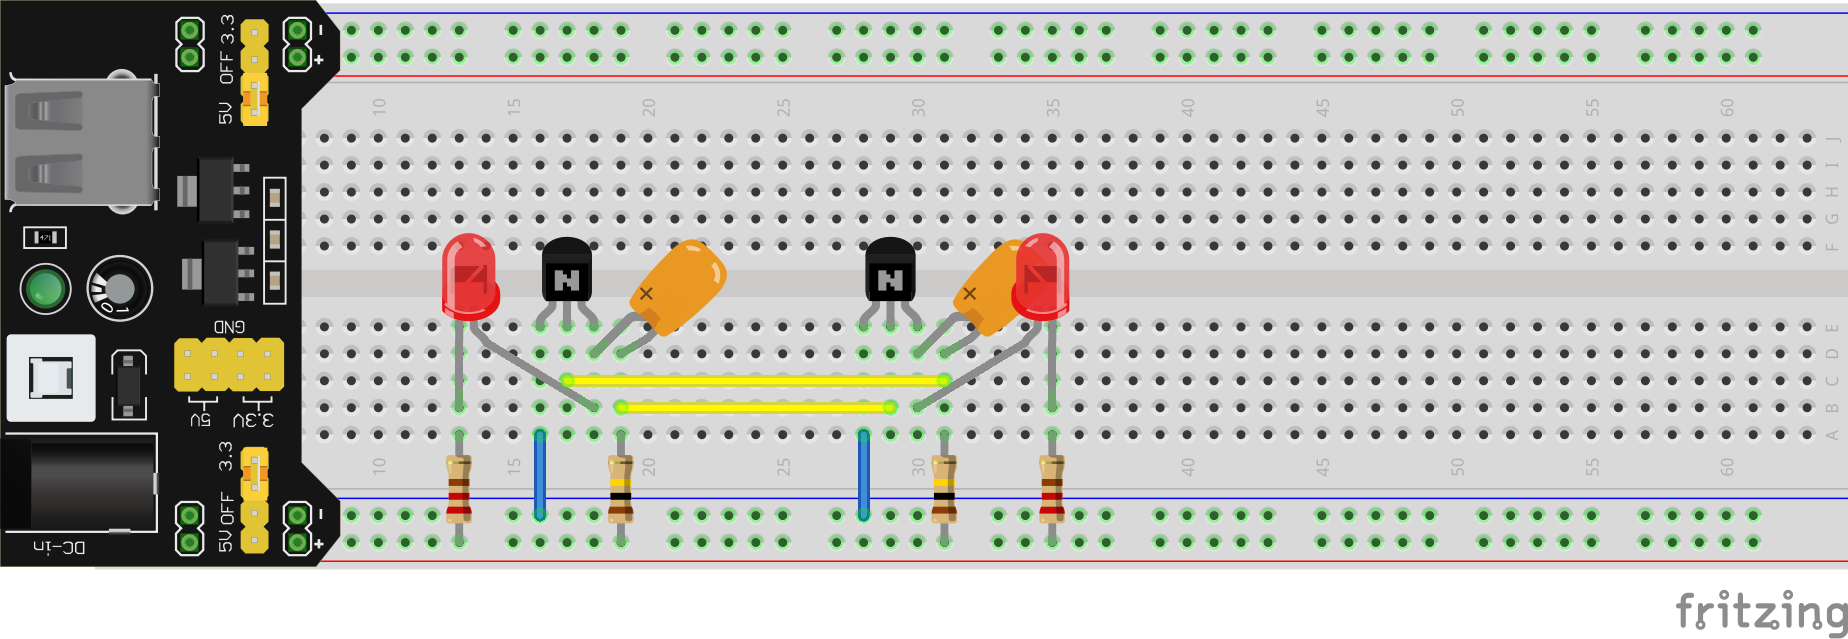
\includegraphics[width=0.8\textwidth]{lesson_circuits/L4/lesson_4.png}
    \caption{Circuit Schematic}
    \label{fig:asm_sch}
\end{figure}
\begin{figure}[!htp]
    \centering
    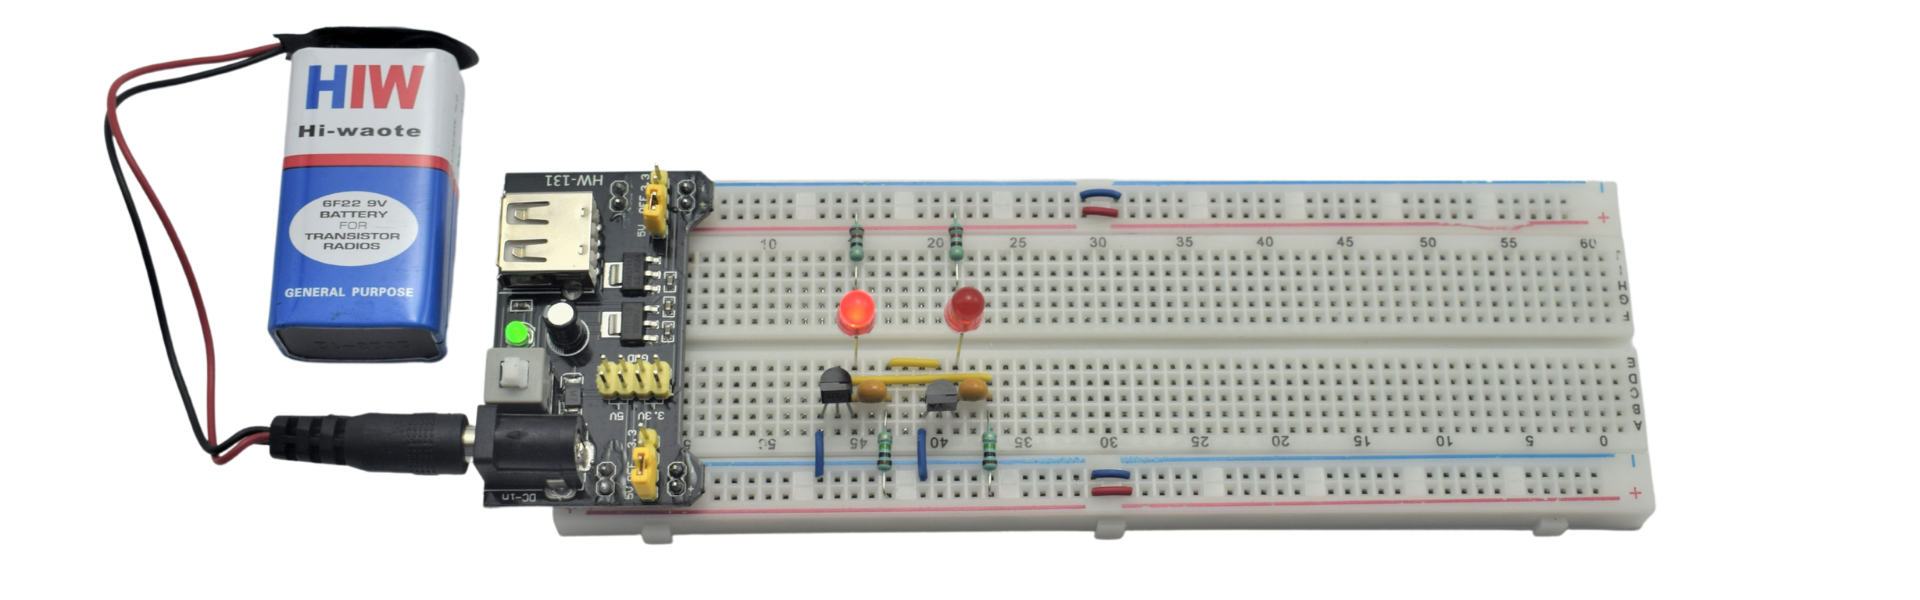
\includegraphics[width=\textwidth]{lesson_circuits/L4/L4-A.png}
    \caption{Astable Multivibrator Breadboard Schematic}
    \label{fig:asm_obb}
\end{figure}



\clearpage
\section{Lesson 5: Transistor as Touch Sensor}
\subsection{Objective}
In this activity we will build a very basic touch sensor using transistors.
\subsection{Components Required}
\begin{enumerate}
    \item Breadboard Power Supply $\times$ 1
    \item 9V Battery $\times$ 1
    \item 9V Battery Connector $\times$ 1
    \item Breadboard $\times$ 1
    \item Red LED $\times$ 1
    \item \SI{220}{\ohm} $\times$ 1
    \item \SI{10}{\kilo\ohm} $\times$ 1
    \item 2N2222 NPN Transistor $\times$ 2
    \item Male pin header $\times$ 2
    \item Male-Male jumper wire $\times$ 5
\end{enumerate}
\subsection{Circuit}
\begin{figure}[!htp]
    \centering
    \begin{circuitikz}[scale = 2]
        \draw (0,0) node[npn](npn1){$T2=2N2222$};
        \draw (npn1.E) node[ground]{};
        \draw (-2,1.5) node[npn](npn2){$T1=2N2222$};
        \draw (npn1.B) to[R, l^=$\SI{10}{\kilo\ohm}$] ++(-1,0) -| (npn2.E);
        \draw ($(npn1.C)+(0,3)$) node[vcc](vcc1){VCC=\SI{5}{\volt}} to[R, l=$\SI{220}{\ohm}$] ($(npn1.C)+(0,2)$)
        to[empty led] (npn1.C);
        \draw (npn2.C) -| ++(0,1.5) to[short, -*] (vcc1);
        \draw (npn2.B) to[short, -o] ++(-0.57,0);
        \draw (npn2.C) to[short, *-o] ++(-1,0);
        \node[left=40,above=4] at (npn2.B) {Touch};
    \end{circuitikz}
    \caption{Transistors as Touch Sensor}
    \label{fig:transistor_touch_circuit}
\end{figure}
\subsection{Circuit Explanation}
By default both the transistors are turned off. When you touch the male pin headers connected between $VCC$ and the base of $T1$, you body acts like a resistor between them, allowing a very small current($I_{B1}$) to pass through the base of $T1$. This current is not sufficient to push $T1$ into saturation.

Therefore, we have connected the base of $T2$ to the emitter of $T1$ and the base current($I_{B2}$) for $T2$ is approximately equal to the collector current($I_{C1}$) of $T1$, which is $\beta \times I_{B1}$. This current is sufficient to pull the $T2$ transistor into saturation mode and the LED turn on.
\begin{figure}[!htp]
    \centering
    \begin{circuitikz}[scale = 2]
        \draw (0,0) node[npn](npn1){$2N2222$};
        \draw (npn1.E) node[ground](gnd1){};
        \draw (-2,1.5) node[npn](npn2){$2N2222$};
        \draw (npn1.B) to[R, l^=$\SI{10}{\kilo\ohm}$] ++(-1,0) -| (npn2.E);
        \draw ($(npn1.C)+(0,3)$) node[vcc](vcc1){VCC=\SI{5}{\volt}} to[R, l=$\SI{220}{\ohm}$] ($(npn1.C)+(0,2)$)
        to[empty led] (npn1.C);
        \draw (npn2.C) -| ++(0,1.5) to[short, -*] (vcc1);
        \draw (npn2.B) to[short, -o] ++(-0.57,0);
        \draw (npn2.C) to[short, *-o] ++(-1,0);
        \draw[red] ($(npn2.C)+(-1,0)$) -- ++(0,0.5)
                to[short, -o] ++(-1,0) 
                node[](T1){};
        \draw[red] ($(npn2.B)+(-0.57,0)$) -- ++(0,-0.5)
                to[short, -o] ++(-1,0)
                node[](T2){};
        \draw[red] (T1) to[R, l_=$R_{Body}$] (T2);
        \node[left=40,above=4] at (npn2.B) {Touch};
        \draw[-latex, orange]
            ($(T2)+(0,-0.2)$) -- ++(1.2,0)
            -- ++(0,0.5) -- ++(0.5,0) node[midway,below]{$I_{B1}$};
        \draw[-latex, green]
            ($(npn2.E)-(0.2,0.2)$) |- ($(npn1.B)+(0,0.2)$)
            node[midway,above left, text width=6mm]{$I_{B2}$ $I_{C1}$};
        \draw[-latex, red]
            ($(vcc1)+(0.3,0)$) -- ($(gnd1)+(0.3,0)$)
            node[midway,right]{$I_{C2}$};
    \end{circuitikz}
    \caption{Touch Sensor Working}
    \label{fig:transistor_touch_working}
\end{figure}
\subsection{Circuit Picture}
\begin{figure}[!htp]
    \centering
    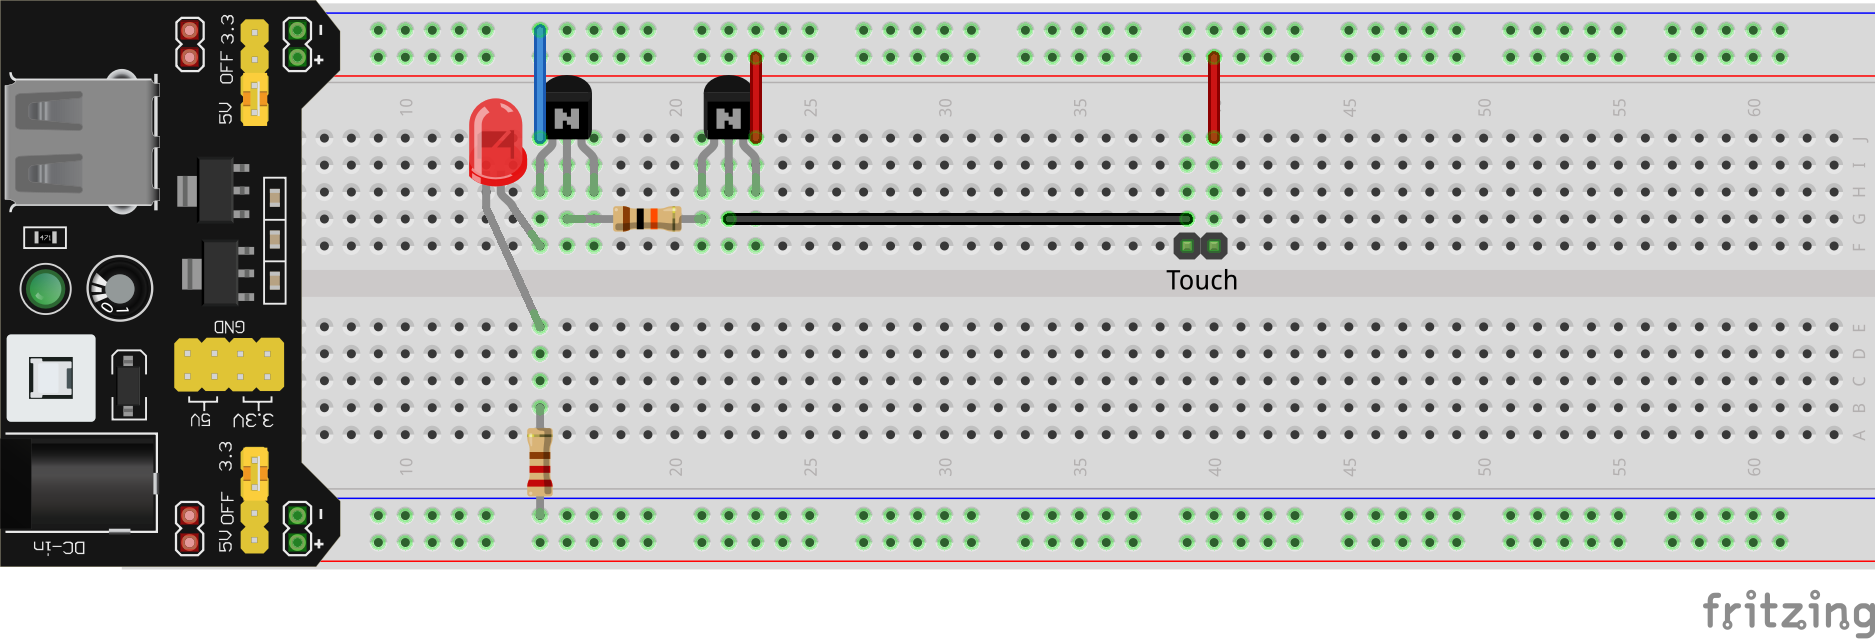
\includegraphics[width=0.8\textwidth]{lesson_circuits/L5/lesson_5.png}
    \caption{Breadboard Schematic}
    \label{fig:simple_touch_sch}
\end{figure}
\begin{figure}[!htp]
    \centering
    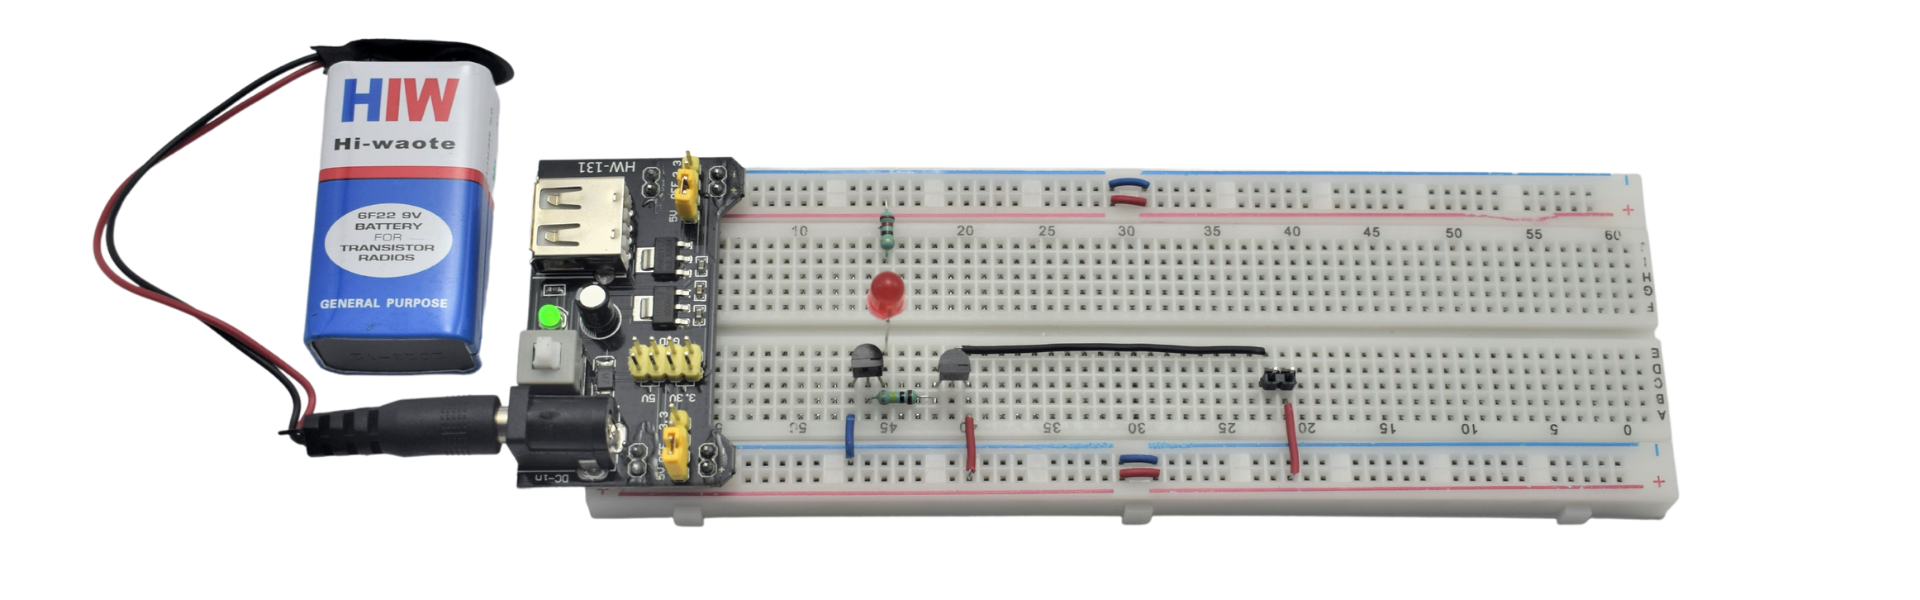
\includegraphics[width=\textwidth]{lesson_circuits/L5/L5-A.png}
    \caption{Touch Switch on Breadboard}
    \label{fig:stouch_obb}
\end{figure}
\begin{figure}[!htp]
    \centering
    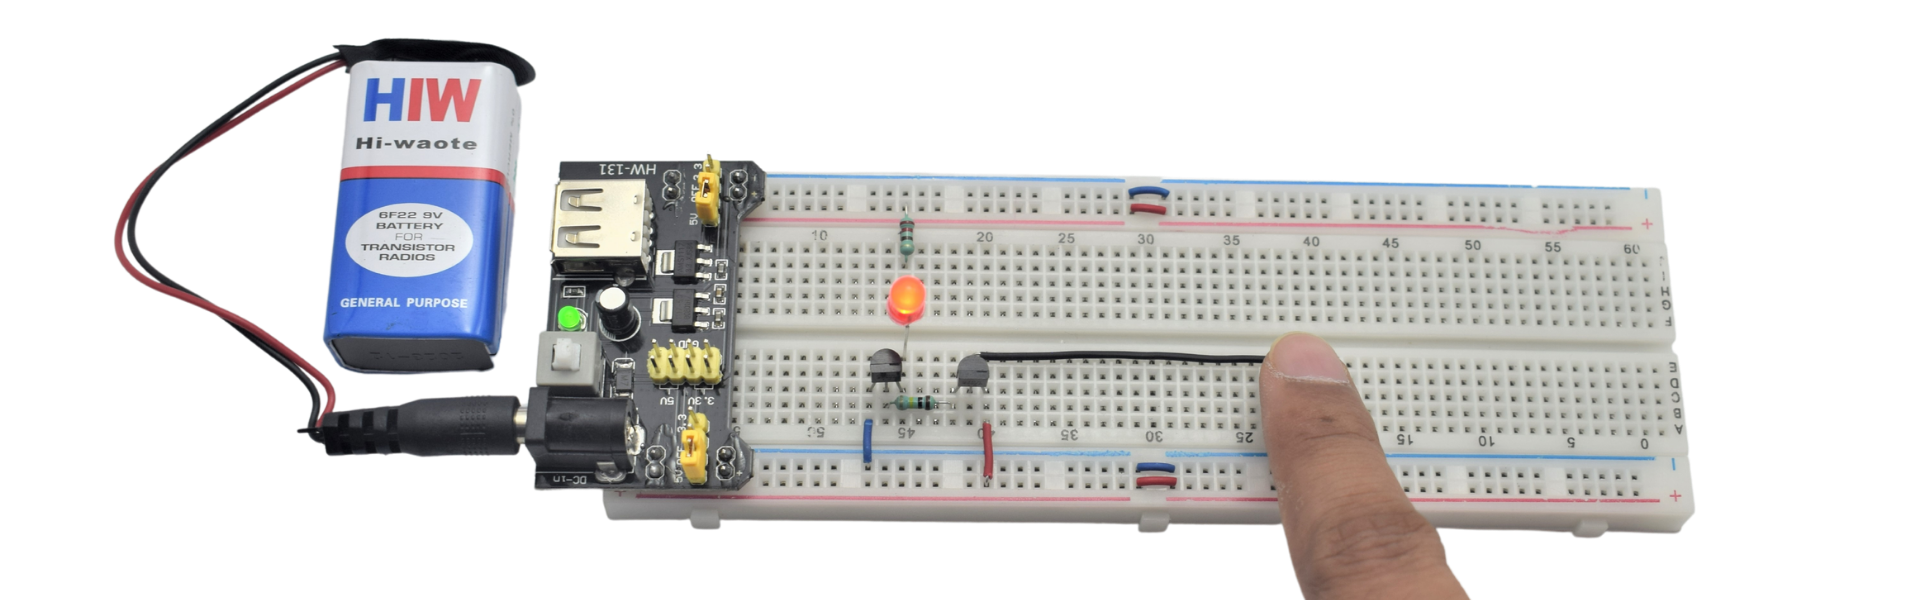
\includegraphics[width=\textwidth]{lesson_circuits/L5/L5-B.png}
    \caption{Touch Switch on Breadboard - LED glows on touching the pin headers}
    \label{fig:stouch_on_obb} 
\end{figure}


\clearpage
\section{Lesson 6: Flip Flop}
\subsection{Objective}
In this activity we'll use transistors and push buttons to make a flip flop circuit.
\subsection{Components Required}
\begin{enumerate}
    \item Breadboard Power Supply $\times$ 1
    \item 9V Battery $\times$ 1
    \item 9V Battery Connector $\times$ 1
    \item Breadboard $\times$ 1
    \item Red LED $\times$ 2
    \item \SI{1}{\kilo\ohm} $\times$ 2
    \item \SI{100}{\kilo\ohm} $\times$ 2
    \item 2N2222 NPN Transistor $\times$ 2
    \item 10-XX Push Buttons $\times$ 2
    \item Male-Male jumper wire $\times$ 8
\end{enumerate}
\subsection{Circuit}
\begin{figure}[!htp]
    \centering
    \begin{circuitikz}[scale = 2]
        \draw (2, 0) node[npn](npn1){$T_1=2N2222$};
        \draw ( -2, 0) node[npn, xscale=-1](npn2){\scalebox{-1}[1]{$T_2=2N2222$}};
        \draw (npn2.E) to[short, -*] ++(1.5,0)
                to[short, -*] ++(0.5,0)
                node[ground]{}
                to[short, -*] ++(0.5,0)
                to[short] (npn1.E);
        \draw (npn1.C) -- ++(0,1)
                to[empty led, invert, mirror, l=$L_1$] ++(0,1)
                to[R, l=$\SI{1}{\kilo\ohm}$] ++(0,1) -- ++(-2,0);
        \draw (npn2.C) -- ++(0,1)
                to[empty led, invert, l_=$L_2$] ++(0,1)
                to[R, l=$\SI{1}{\kilo\ohm}$] ++(0,1)
                to[short, -*] ++(2,0)
                node[vcc]{VCC};
        \draw[orange] ($(npn2.E)+(1.5,0)$) to[push button, l=$B_2$] ++(0,1)
                    |- ++(1,0.5)
                    to[R, l=$\SI{100}{\kilo\ohm}$] ++(1,0) 
                    to[short,-*] ++(0.5,0);
        \draw[red] ($(npn1.E)-(1.5,0)$) to[push button, mirror, l_=$B_1$] ++(0,1)
                    |- ++(-1,0.7)
                    to[R, l_=$\SI{100}{\kilo\ohm}$] ++(-1,0) 
                    to[short,-*] ++(-0.5,0);
        \draw[orange] (npn2.B) -| ++(0.5,0.7)
                    to[short, -*] ++(0.575,0);
        \draw[red] (npn1.B) -| ++(-0.5,0.7)
            to[short, -*] ++(-0.575,0);
    \end{circuitikz}
    \caption{Flip Flop}
    \label{fig:flip_flop}
\end{figure}
\subsection{Circuit Explanation}
Let's assume that $L_1$ is on, which means there is a very small amount of current flowing through the $L_2$ to the base of transistor $T_1$. The current flowing through $L_1$ will prefer to go through the transistor $T_1$ because this path offers the least resistance.

Now, when we press the button $B_1$ the current going to the base of $T_1$ will now directly go to the ground, switching $T_1$ off. And there will be a small current going through the led $L_1$ to the base of transistor $T_2$, pushing it into saturation. And when we leave the button $B_1$ the current through $L_2$ will go through $T_2$ only, as it will offer a path with least resistance.
\begin{figure}[!htp]
    \centering
    \begin{circuitikz}[scale = 2]
        \draw (2, 0) node[npn](npn1){$T_1=2N2222$};
        \draw ( -2, 0) node[npn, xscale=-1](npn2){\scalebox{-1}[1]{$T_2=2N2222$}};
        \draw (npn2.E) to[short, -*] ++(1.5,0)
                to[short, -*] ++(0.5,0)
                node[ground]{}
                to[short, -*] ++(0.5,0)
                to[short] (npn1.E);
        \draw (npn1.C) -- ++(0,1)
                to[empty led, invert, mirror, l=$L_1$] ++(0,1)
                to[R, l=$\SI{1}{\kilo\ohm}$] ++(0,1) -- ++(-2,0);
        \draw (npn2.C) -- ++(0,1)
                to[empty led, invert, color=red, l_=$L_2$] ++(0,1)
                to[R, l_=$\SI{1}{\kilo\ohm}$] ++(0,1)
                to[short, -*] ++(2,0)
                node[vcc]{VCC};
        \draw[orange] ($(npn2.E)+(1.5,0)$) to[push button, l=$B_2$] ++(0,1)
                    |- ++(1,0.5)
                    to[R, l=$\SI{100}{\kilo\ohm}$] ++(1,0) 
                    to[short,-*] ++(0.5,0);
        \draw[red] ($(npn1.E)-(1.5,0)$) to[normally closed push button, mirror, l_=$B_1$] ++(0,1)
                    |- ++(-1,0.7)
                    to[R, l_=$\SI{100}{\kilo\ohm}$] ++(-1,0) 
                    to[short,-*] ++(-0.5,0);
        \draw[orange] (npn2.B) -| ++(0.5,0.7)
                    to[short, -*] ++(0.575,0);
        \draw[red] (npn1.B) -| ++(-0.5,0.7)
            to[short, -*] ++(-0.575,0);
        \draw[-latex, color=brown] 
            (2.4, 3.2) -- (2.4, 0.9) -- (-1.3,0.9) -- (-1.3,0.2) -- (-1.5,0.2);
        \draw[-latex, color=red] 
            (-2.4, 3.2) to[short,-*] (-2.4, 1.15) -- (0.3,1.15) -- (0.3,0);
        \draw[-latex, color=red] 
            (-2.4, 3.2) -- (-2.4, 0);
    \end{circuitikz}
    \caption{Flip Flop Working}
    \label{fig:flip_flop_working}
\end{figure}
\subsection{Circuit Picture}
\begin{figure}[!htp]
    \centering
    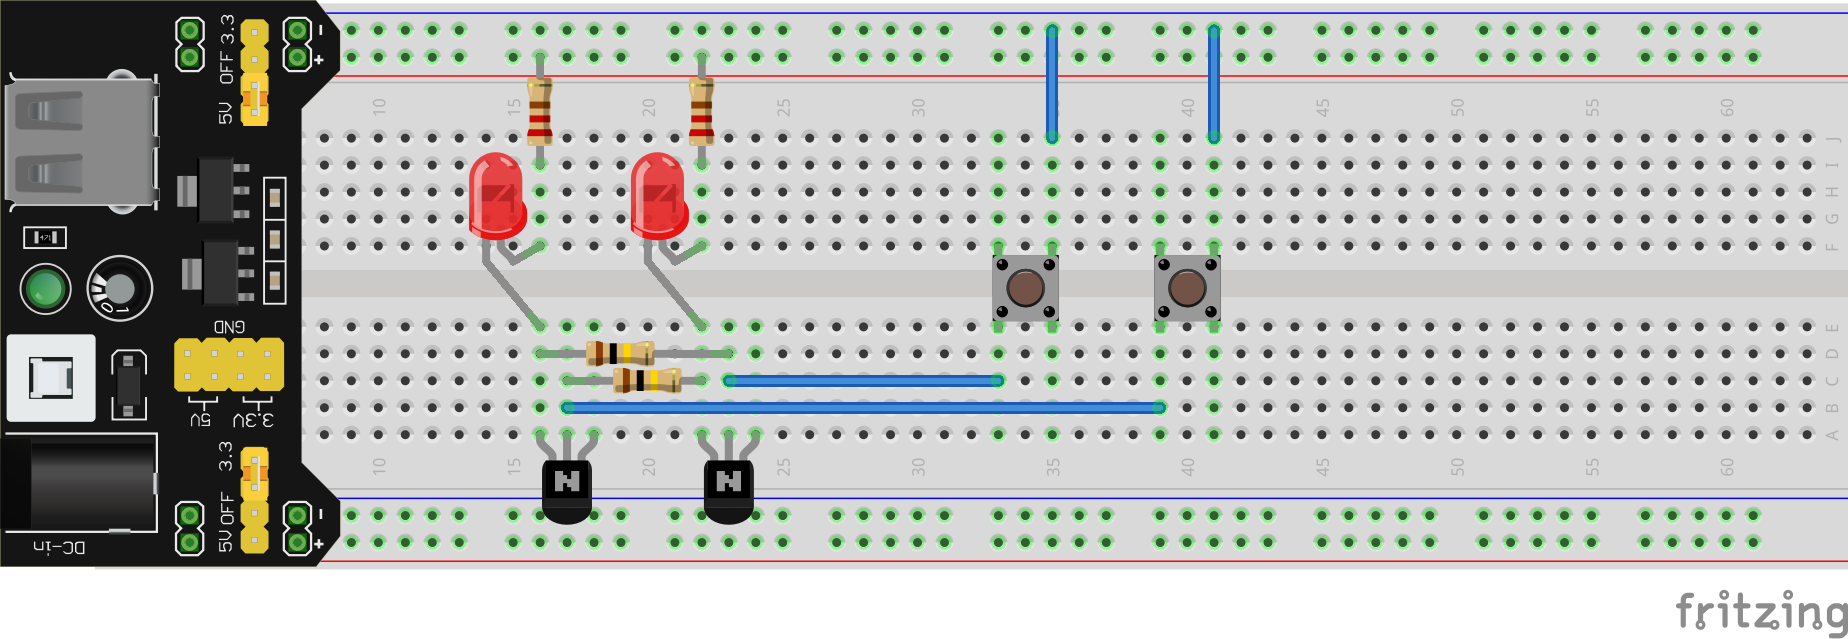
\includegraphics[width=0.8\textwidth]{lesson_circuits/L6/lesson_6.png}
    \caption{Breadboard Schematic}
    \label{fig:ff_bjt_sch}
\end{figure}
\begin{figure}[!htp]
    \centering
    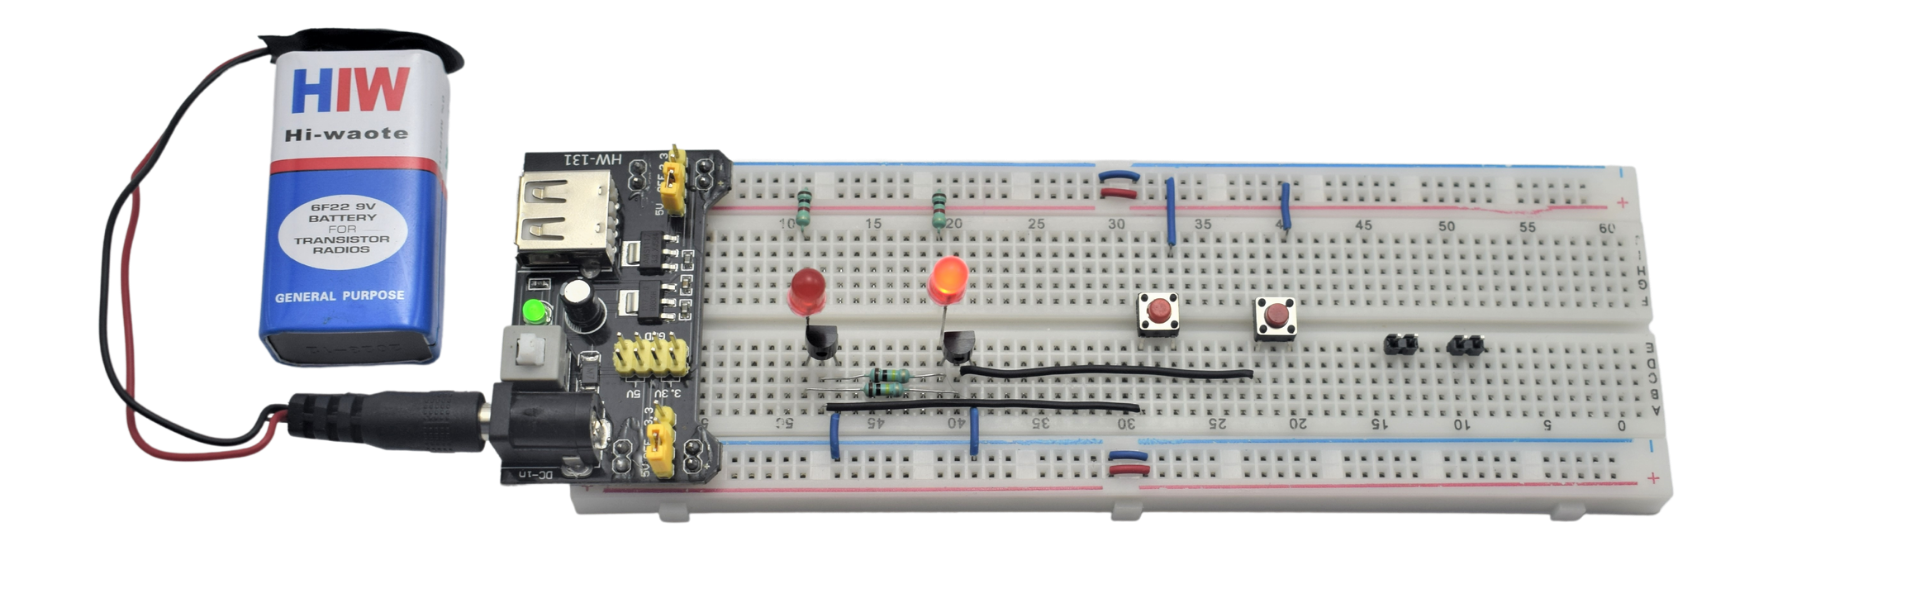
\includegraphics[width=\textwidth]{lesson_circuits/L6/L6-A.png}
    \caption{Flip/Flop using BJTs on Breadboard}
    \label{fig:ff_obb1}
\end{figure}
\begin{figure}[!htp]
    \centering
    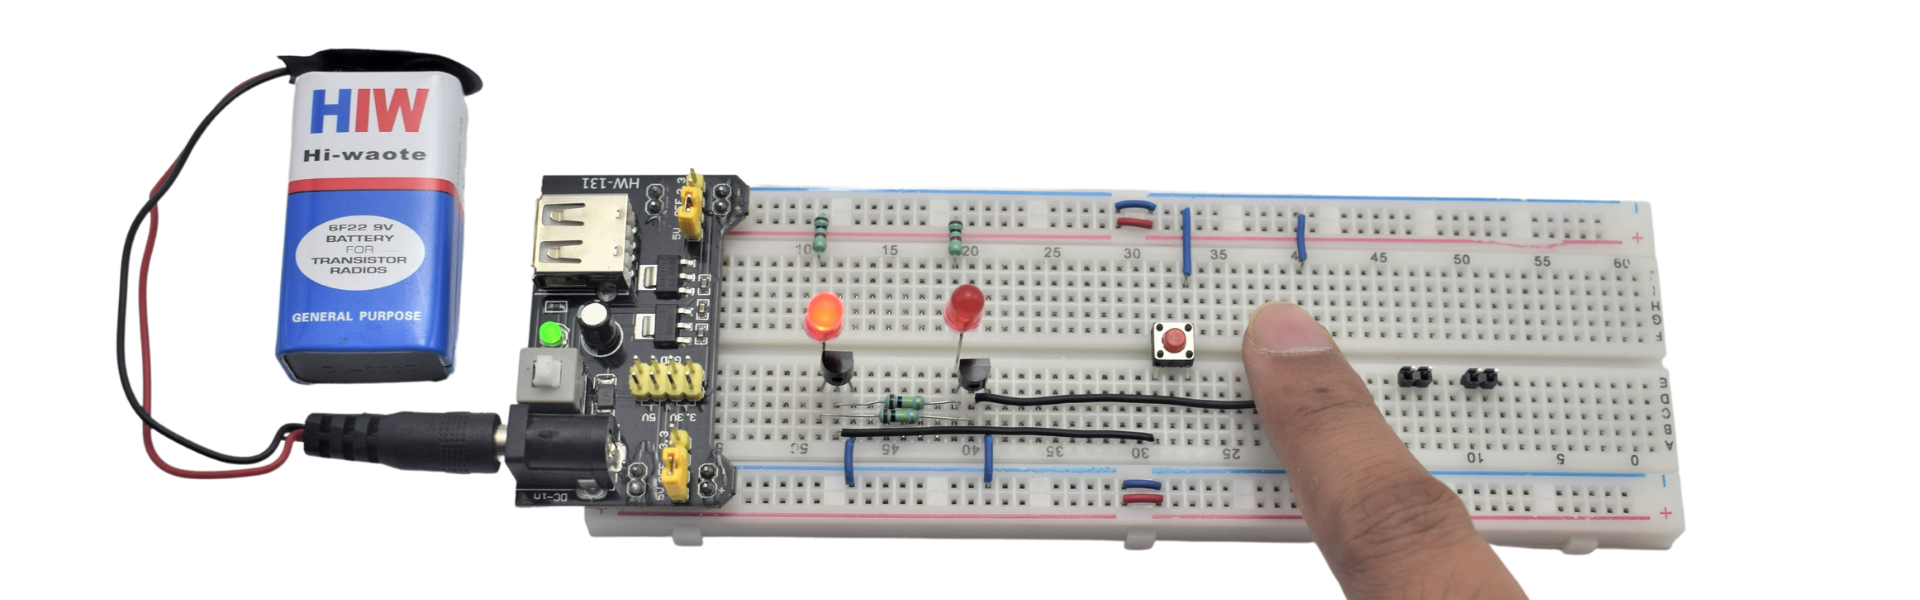
\includegraphics[width=\textwidth]{lesson_circuits/L6/L6-B.png}
    \caption{Flip/Flop using BJTs on Breadboard}
    \label{fig:ff_obb2}
\end{figure}
\begin{figure}[!htp]
    \centering
    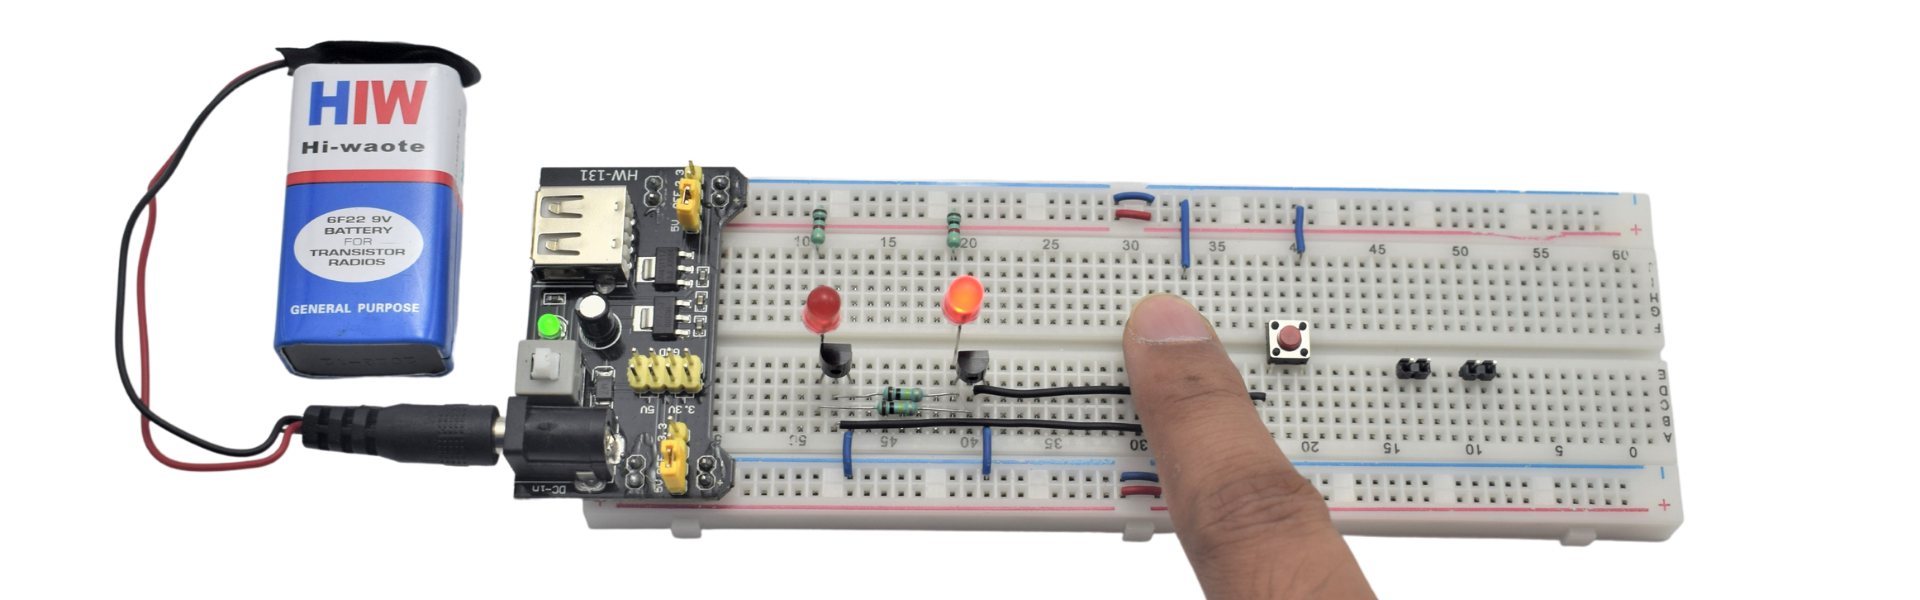
\includegraphics[width=\textwidth]{lesson_circuits/L6/L6-C.png}
    \caption{Flip/Flop using BJTs on Breadboard}
    \label{fig:ff_obb3}
\end{figure}
\begin{figure}[!htp]
    \centering
    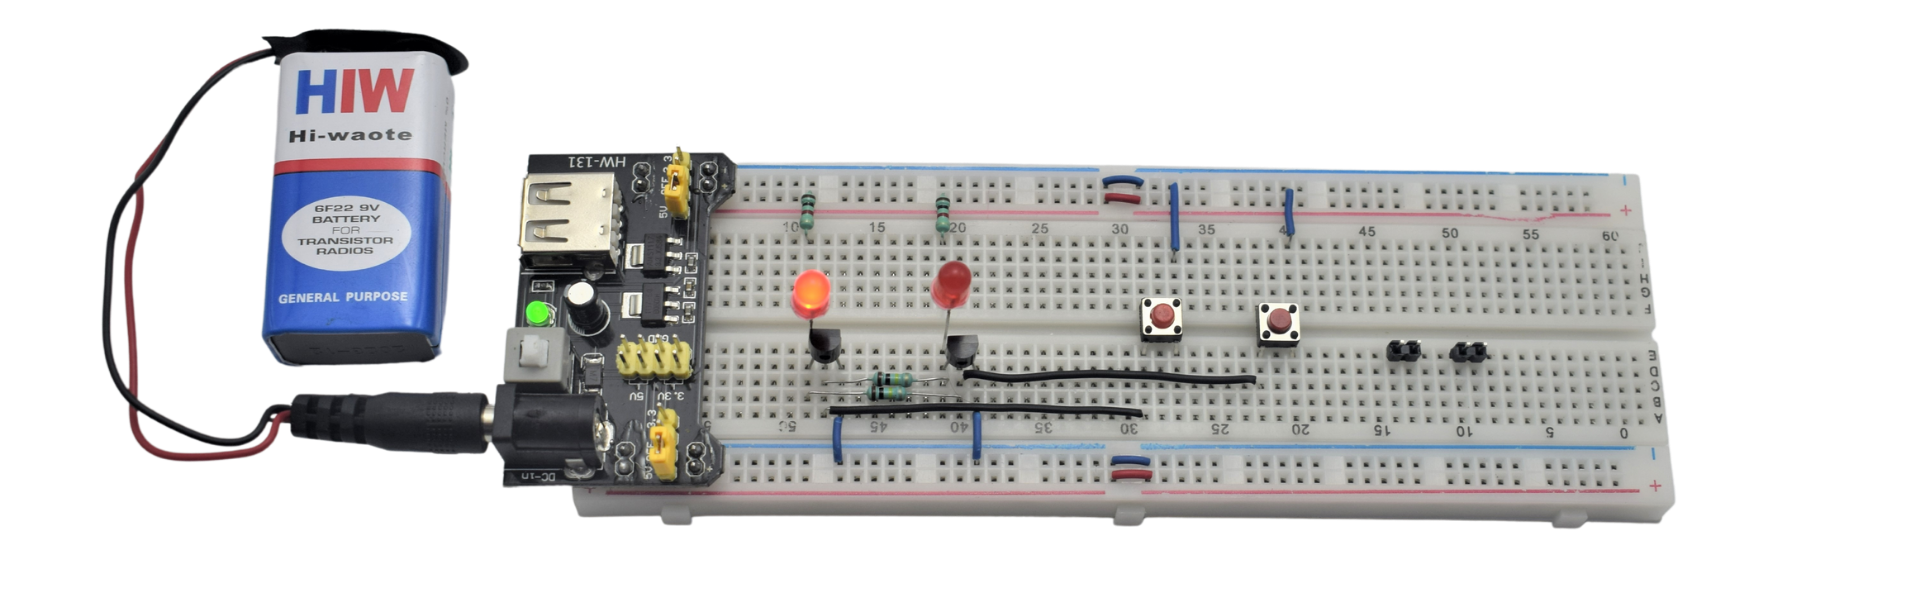
\includegraphics[width=\textwidth]{lesson_circuits/L6/L6-D.png}
    \caption{Flip/Flop using BJTs on Breadboard}
    \label{fig:ff_obb4}
\end{figure}


\clearpage
\section{Lesson 7: On/Off Touch using Transistors}
\subsection{Objective}
In this activity we will make an on off touch switch using transistors, which will remember its state.
\subsection{Components Required}
\begin{enumerate}
    \item Breadboard Power Supply $\times$ 1
    \item 9V Battery $\times$ 1
    \item 9V Battery Connector $\times$ 1
    \item Breadboard $\times$ 1
    \item Red LED $\times$ 1
    \item \SI{220}{\ohm} $\times$ 1
    \item \SI{10}{\kilo\ohm} $\times$ 1
    \item \SI{100}{\kilo\ohm} $\times$ 1
    \item 2N2222 NPN Transistor $\times$ 3
    \item 2N2907 PNP Transistor $\times$ 1
    \item Male pin headers $\times$ 4
    \item Male-Male jumper wire $\times$ 13
\end{enumerate}
\subsection{Circuit}
\begin{figure}[!htp]
    \centering
    \begin{circuitikz}[scale = 2]
        \draw (1.5,3) node[pnp](t1){T1};
        \draw (0,2.5) node[npn](t2){T2};
        \draw (-1,2) node[npn](t3){T3};
        \draw (-2,3.5) node[npn](t4){T4};
        \draw (t3.E) |- (0,0)
                node[ground]{} 
                to[short, *-] (t2.E);
        \draw (0,0) -- (1.5,0)
                to[empty led, invert, mirror] ++(0,0.75);
        \draw[red] (1.5,0.75) to[R, l_=$\SI{200}{\ohm}$] ++(0,0.75)
                to[short, *-] (t1.C);
        \draw[purple] (1.5,1.5) to[R, l^=$\SI{100}{\kilo\ohm}$] ++(-2,0)
                to[short, -*] ++(0,1);
        \draw[purple] (t3.C) to[short, -*] ++(0,0.11);
        \draw[purple] (t2.B) to[short, -o] ++(-4,0);
        \draw[green] (t4.E) |- (t3.B);
        \draw[green] (t4.B) to[short, -o] ++(-2,0);
        \draw[red] (t1.E) |- (0,4) node[vcc](vcc1){VCC};
        \draw[red] (vcc1) to[short, *-*] (-2,4) -- (t4.C);
        \draw[red] (-2,4) -- (-3,4)
                to[short, -*] (-3,3.7) 
                to[short, -o] ++(-1.42,0);
        \draw[red] (-3, 3.7) -- (-3,2.7)
                to[short, -o] ++(-1.42,0);
        \draw (vcc1) to[R, l=$\SI{10}{\kilo\ohm}$] (t2.C);
        \draw[blue] (t1.B) to[short, -*] (0,3);
        \draw[green] (-4.7,3.6) node[]{OFF};
        \draw[red] (-4.7,2.6) node[]{ON};
    \end{circuitikz}
    \caption{On/Off Touch Switch using Transistors}
    \label{fig:on_off_transistor}
\end{figure}
\subsection{Circuit Explanation}
When we touch the pin headers marked \emph{on}, we introduce our body resistance between $VCC$ and base of transistor $T2$, turning it on. When $T2$ is turned on, it pulls the base of transistor $T1$ to ground, pushing it to saturation mode. A small part of the current flowing through the collector of $T1$ goes to the base of $T2$ through feedback resistor. Now, when we remove our body resistance from the circuit the current through feedback keeps $T2$ on, which make sure the $T1$ is on and the led is glowing.
\begin{figure}[!htp]
    \centering
    \begin{circuitikz}[scale = 2]
        \draw (1.5,3) node[pnp](t1){T1};
        \draw (0,2.5) node[npn](t2){T2};
        \draw (-1,2) node[npn](t3){T3};
        \draw (-2,3.5) node[npn](t4){T4};
        \draw (t3.E) |- (0,0)
                node[ground]{} 
                to[short, *-] (t2.E);
        \draw (0,0) -- (1.5,0)
                to[empty led, invert, mirror] ++(0,0.75);
        \draw[red] (1.5,0.75) to[R, l_=$\SI{200}{\ohm}$] ++(0,0.75)
                to[short, *-] (t1.C);
        \draw[purple] (1.5,1.5) to[R, l^=$\SI{100}{\kilo\ohm}$] ++(-2,0)
                to[short, -*] ++(0,1);
        \draw[purple] (t3.C) to[short, -*] ++(0,0.11);
        \draw[purple] (t2.B) to[short, -o] ++(-3,0)  node[](o1){};
        \draw[green] (t4.E) |- (t3.B);
        \draw[green] (t4.B) to[short, -o] ++(-2,0);
        \draw[red] (t1.E) |- (0,4) node[vcc](vcc1){VCC};
        \draw[red] (vcc1) to[short, *-*] (-2,4) -- (t4.C);
        \draw[red] (-2,4) -- (-3,4)
                to[short, -*] (-3,3.7) 
                to[short, -o] ++(-1.42,0);
        \draw[red] (-3, 3.7) -- (-3,2.7)
                to[short, -o] ++(-0.42,0) node[](o2){};
        \draw (vcc1) to[R, l=$\SI{10}{\kilo\ohm}$] (t2.C);
        \draw[blue] (t1.B) to[short, -*] (0,3);
        \draw[green] (-4.7,3.6) node[]{OFF};
        \draw[red] (-3.7,2.6) node[]{ON};
        \draw[red]
            (o2) -- ++(0,0.5) 
            to[short, -o] ++(-1,0) node[](r1){};
        \draw[red]
            (o1) -- ++(0,-0.5) 
            to[short, -o] ++(-1,0) node[](r2){};
        \draw[red]
            (r1) to[R, l_=$R_{Body}$] (r2);
        \draw[-latex, brown]
            ($(r2)+(0,-0.2)$) -- ++(1.2,0) -- ++(0,0.5) -- ++(2.9,0) node[midway,below=3mm,left=6mm]{$I_{B2}$};
        \draw[-latex, orange]
            ($(t1.E)+(0.3,0)$) to[short,-*] ++(0,-1.6) -- ++(0,-1.3) node[midway, right=4mm, above=6mm]{$I_{led}$};
        \draw[-latex, orange]
            ($(t1.E)+(0.3,-1.6)$) -- ++(-2,0) -- ++(0,0.5) node[midway,right =8mm]{$I_{feedback}$};
    \end{circuitikz}
    \caption{Touch Switch using Transistors - On State}
    \label{fig:on_off_transistor_on_working}
\end{figure}

Now, when we touch the pin header marked \emph{off}, we introduce our body resistance in between the $VCC$ and the base of $T4$, turning it on. The $T4$ collector current goes to the base of $T3$, turning it on. There are two things that causes the led to turn off, base of $T2$ is pulled to ground, and the feedback current keeping it on goes to ground via $T3$. It means $T2$ is switched off, and when $T2$ is off the base of $T1$ is pulled high, turning it hard off.
\begin{figure}[!htp]
    \centering
    \begin{circuitikz}[scale = 2]
        \draw (1.5,3) node[pnp](t1){T1};
        \draw (0,2.5) node[npn](t2){T2};
        \draw (-1,2) node[npn](t3){T3};
        \draw (-2,3.5) node[npn](t4){T4};
        \draw (t3.E) |- (0,0)
                node[ground]{} 
                to[short, *-] (t2.E);
        \draw (0,0) -- (1.5,0)
                to[empty led, invert, mirror] ++(0,0.75);
        \draw[red] (1.5,0.75) to[R, l_=$\SI{200}{\ohm}$] ++(0,0.75)
                to[short, *-] (t1.C);
        \draw[purple] (1.5,1.5) to[R, l^=$\SI{100}{\kilo\ohm}$] ++(-2,0)
                to[short, -*] ++(0,1);
        \draw[purple] (t3.C) to[short, -*] ++(0,0.11);
        \draw[purple] (t2.B) to[short, -o] ++(-4,0);
        \draw[green] (t4.E) |- (t3.B);
        \draw[green] (t4.B) to[short, -o] ++(-1,0) node[](o1){};
        \draw[red] (t1.E) |- (0,4) node[vcc](vcc1){VCC};
        \draw[red] (vcc1) to[short, *-*] (-2,4) -- (t4.C);
        \draw[red] (-2,4) -- (-3,4)
                to[short, -*] (-3,3.7) 
                to[short, -o] ++(-0.42,0) node[](o2){};
        \draw[red] (-3, 3.7) -- (-3,2.7)
                to[short, -o] ++(-1.42,0);
        \draw (vcc1) to[R, l=$\SI{10}{\kilo\ohm}$] (t2.C);
        \draw[blue] (t1.B) to[short, -*] (0,3);
        \draw[green] (-3.7,3.6) node[]{OFF};
        \draw[red] (-4.7,2.6) node[]{ON};
        \draw[red]
            (o2) -- ++(0,0.5) 
            to[short, -o] ++(-1,0) node[](r1){};
        \draw[red]
            (o1) -- ++(0,-0.5) 
            to[short, -o] ++(-1,0) node[](r2){};
        \draw[red]
            (r1) to[R, l_=$R_{Body}$] (r2);
        \draw[-latex, brown]
            ($(r2)+(0,-0.1)$) -- ++(1.1,0) -- ++(0,0.5) -- ++(1,0) node[midway,below=3mm,right=1mm]{$I_{B4}$};
        \draw[-latex, brown]
            ($(t4.E)+(0.2,0)$) -- ++(0,-0.9) -- ++(0.5,0);
        \draw[-latex, orange]
            ($(t3.E)+(-0.2,0)$) -- ++(0,-1.5)
            node[midway, left=4mm, above=1mm]{$I_{C3}$};
        \draw[-latex, orange]
            ($(t1.E)+(0.2,-1.7)$) -- ++(-2,0) -- ++(0,0.5) node[midway,right =8mm]{$I_{feedback}$}
            -- ++(-0.5,0) -- ++(0,-2);
    \end{circuitikz}
    \caption{Touch Switch using Transistors - Off State}
    \label{fig:on_off_transistor_off_working}
\end{figure}

\subsection{Circuit Picture}
\begin{figure}[!htp]
    \centering
    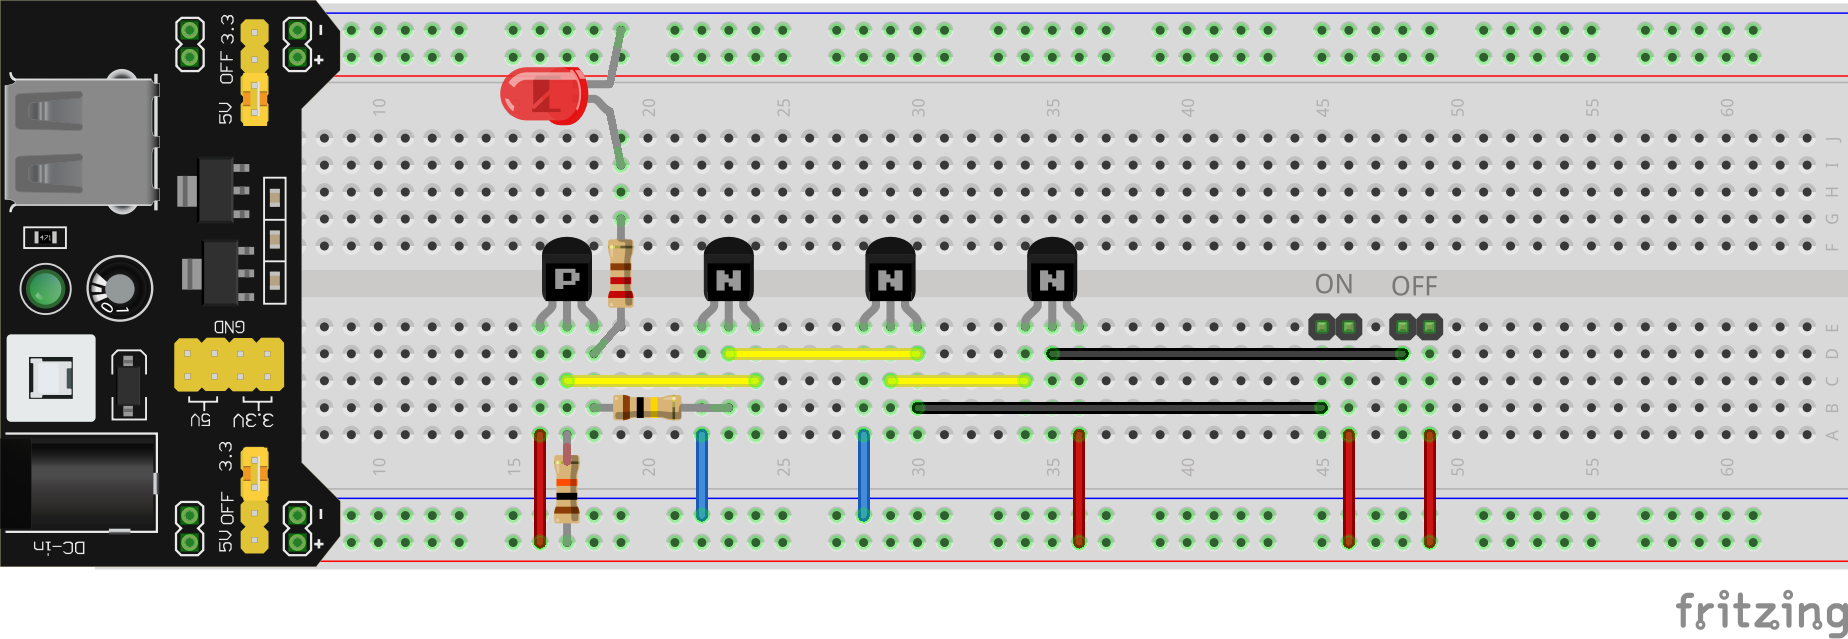
\includegraphics[width=\textwidth]{lesson_circuits/L7/lesson_7.png}
    \caption{On/Off touch switch using BJTs Breadboard Schematic}
    \label{fig:onoff_sch}
\end{figure}
\begin{figure}[!htp]
    \centering
    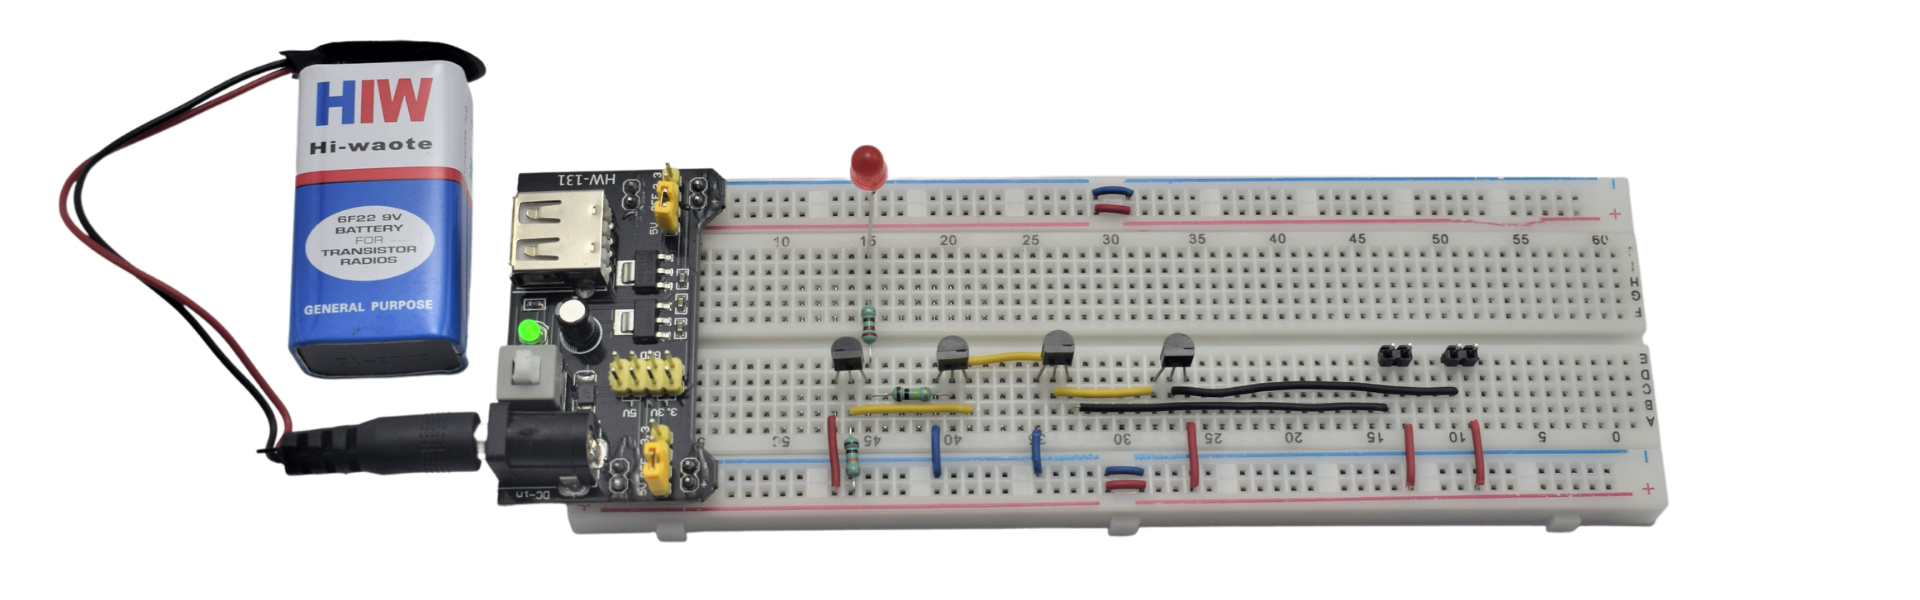
\includegraphics[width=\textwidth]{lesson_circuits/L7/L7-A.png}
    \caption{On/Off Touch Switch: }
    \label{fig:onoff_obb1}
\end{figure}
\begin{figure}[!htp]
    \centering
    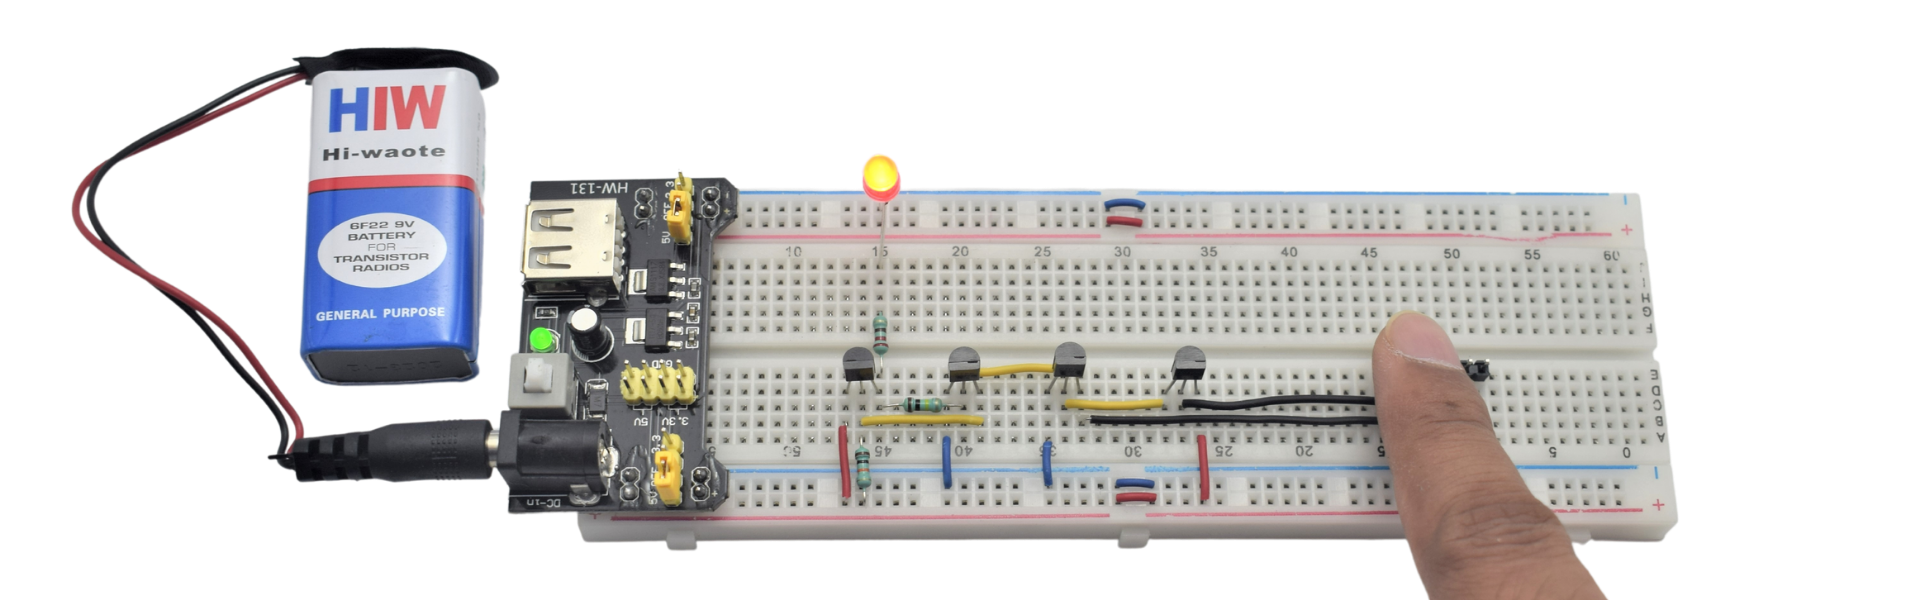
\includegraphics[width=\textwidth]{lesson_circuits/L7/L7-B.png}
    \caption{On/Off Touch Switch: }
    \label{fig:onoff_obb2}
\end{figure}
\begin{figure}[!htp]
    \centering
    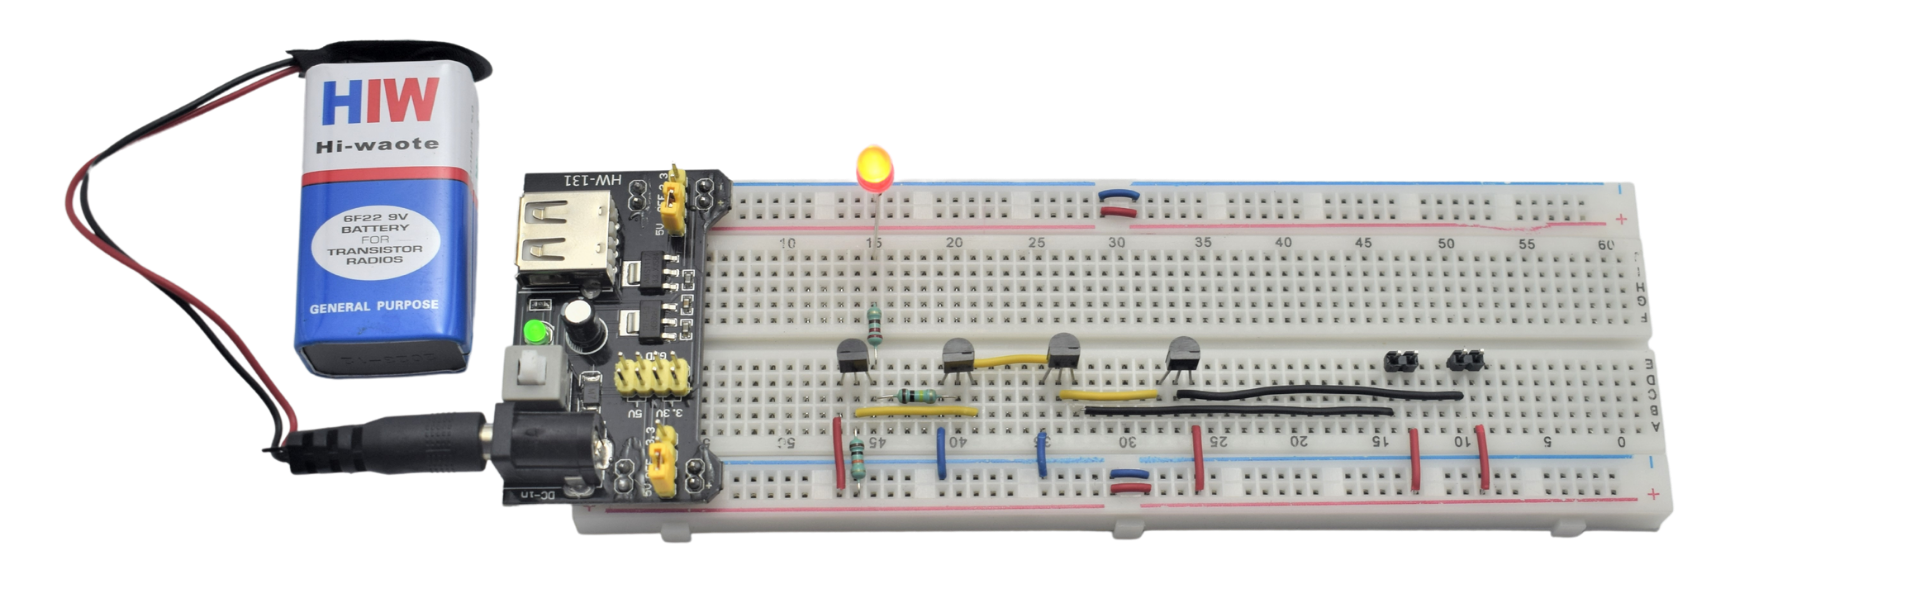
\includegraphics[width=\textwidth]{lesson_circuits/L7/L7-C.png}
    \caption{On/Off Touch Switch: }
    \label{fig:onoff_obb3}
\end{figure}
\begin{figure}[!htp]
    \centering
    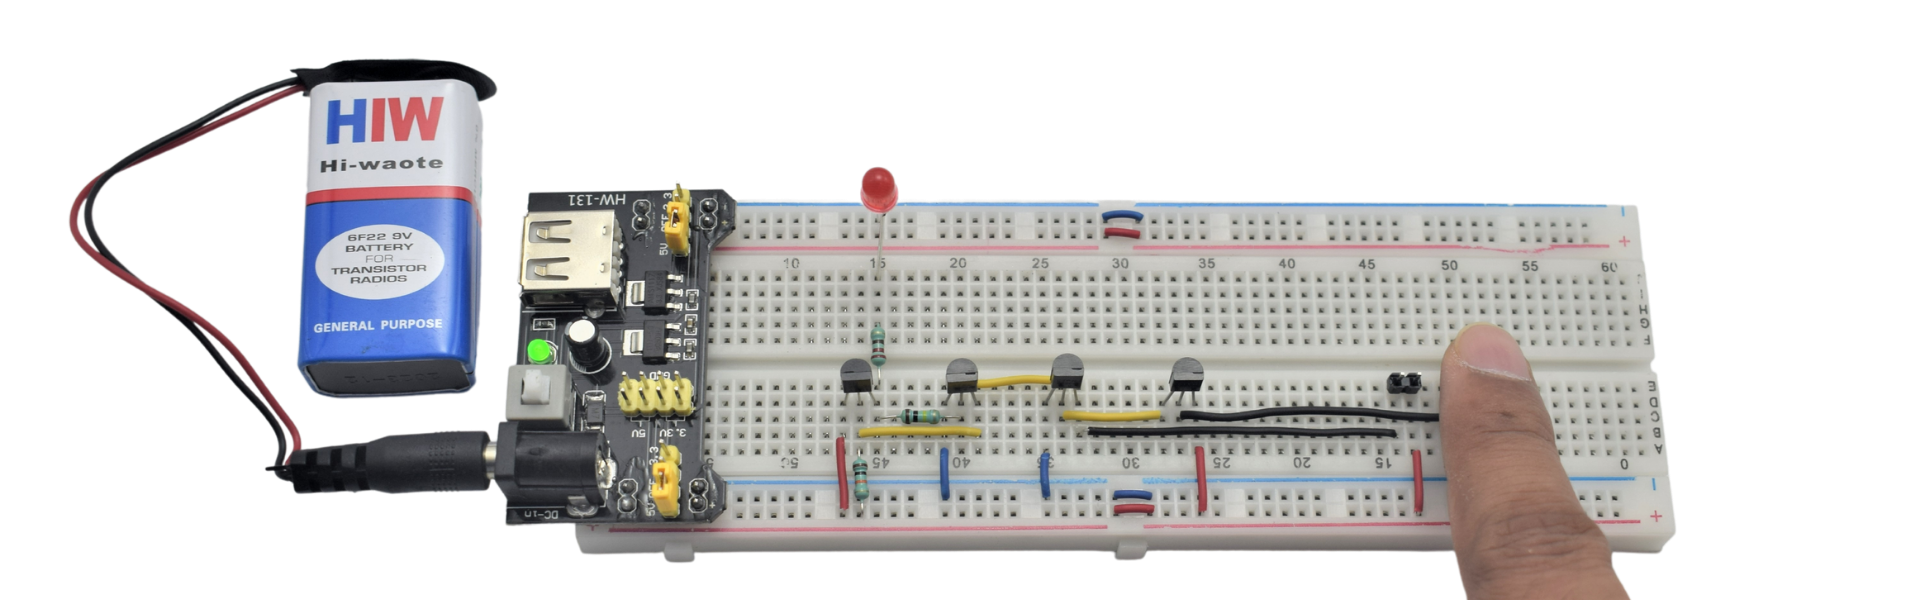
\includegraphics[width=\textwidth]{lesson_circuits/L7/L7-D.png}
    \caption{On/Off Touch Switch: }
    \label{fig:onoff_obb4}
\end{figure}
\begin{figure}[!htp]
    \centering
    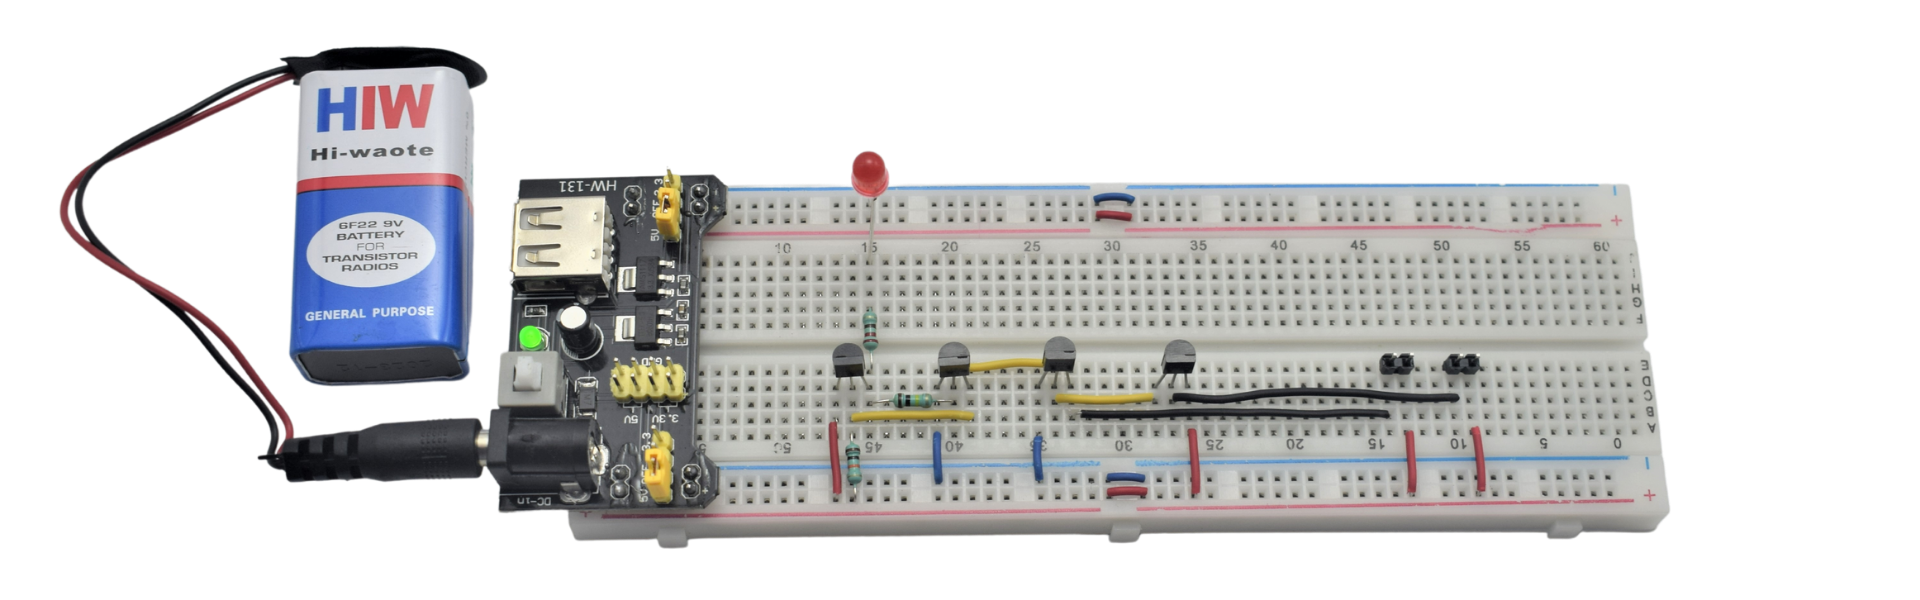
\includegraphics[width=\textwidth]{lesson_circuits/L7/L7-E.png}
    \caption{On/Off Touch Switch: }
    \label{fig:onoff_obb5}
\end{figure}


\clearpage
\section{Lesson 8: Toggle Switch using Transistors}
\subsection{Objective}
In this activity we will make an toggle switch which toggles the output state using push button and transistors.
\subsection{Components Required}
\begin{enumerate}
    \item Breadboard Power Supply $\times$ 1
    \item 9V Battery $\times$ 1
    \item 9V Battery Connector $\times$ 1
    \item Breadboard $\times$ 1
    \item Red LED $\times$ 1
    \item \SI{100}{\nano\farad} $\times$ 1
    \item \SI{220}{\ohm} $\times$ 1
    \item \SI{10}{\kilo\ohm} $\times$ 1
    \item \SI{100}{\kilo\ohm} $\times$ 2
    \item \SI{1}{\mega\ohm} $\times$ 2
    \item 2N2222 NPN Transistor $\times$ 2
    \item 2N2907 PNP Transistor $\times$ 1
    \item 10-XX Push Button $\times$ 1
    \item Male-Male jumper wire $\times$ 10
\end{enumerate}
\subsection{Circuit}
\begin{figure}[!htp]
    \centering
    \begin{circuitikz}[scale = 2]
        \draw (0,2.5) node[npn](t2){T2};
        \draw (2,3) node[pnp](t1){T1};
        \draw (-1.5,1) node[npn, xscale=-1](t3){\scalebox{-1}[1]{T3}};
        \draw (t2.E) to[short, -*] (0,0)
                node[ground](gnd1){};
        \draw (gnd1) -- (2,0)
                to[empty led, invert, mirror] ++(0,1)
                to[R, l_=$\SI{220}{\ohm}$] ++(0,0.7)
                to[short, -*] ++(0,0.2) -- (t1.C);
        \draw[red] (t1.E) -- ++(0,0.5)
                to[short, -*] ++(-2,0) node[vcc](vcc1){5V};
        \draw[red] (vcc1) -| ++(-1.5,-1.5)
                to[R, l=$\SI{1}{\mega\ohm}$] (t3.C);
        \draw (vcc1) to[R, l=$\SI{10}{\kilo\ohm}$] (t2.C);
        \draw[blue] (t1.B) to[short, -*] ++(-1.58,0);
        \draw[green] (t2.B) -- ++(-1,0)
                to[push button, mirror] (-3,2.5) -- ++(0,-1.1);
        \draw (t3.E) to[short, -*] (-1.5,0) -- (gnd1);
        \draw (-1.5,0) -- (-3,0);
        \draw (t3.C) to[short, *-] ++(0,0)
                to[R, l_=$\SI{1}{\mega\ohm}$] ++(-1.5,0)
                to[short, *-] ++(0,0)
                to[C, l=$\SI{100}{\nano\farad}$] (-3,0);
        \draw[orange] (t3.B) to[R, l=$\SI{100}{\kilo\ohm}$] ++(0.7,0) -- ++(2.1,0)
                to[short, -*] ++(0,0.9);
        \draw[purple] (t2.B) to[short, *-] ++(0,-0.6)
                to[R, l=$\SI{100}{\kilo\ohm}$] (2,1.9);
    \end{circuitikz}
    \caption{Toggle Switch using Transistors}
    \label{fig:toggle_transistor}
\end{figure}
\subsection{Circuit Explanation}
Let us assume that initially all the transistors are off along with the led. In this case, the capacitor gets charged via the two $1\si{\mega\ohm}$ resistors. And no current is flowing through any transistor.
\begin{figure}[!htp]
    \centering
    \begin{circuitikz}[scale = 2]
        \draw (0,2.5) node[npn](t2){T2};
        \draw (2,3) node[pnp](t1){T1};
        \draw (-1.5,1) node[npn, xscale=-1](t3){\scalebox{-1}[1]{T3}};
        \draw (t2.E) to[short, -*] (0,0)
                node[ground](gnd1){};
        \draw (gnd1) -- (2,0)
                to[empty led, invert, mirror] ++(0,1)
                to[R, l_=$\SI{220}{\ohm}$] ++(0,0.7)
                to[short, -*] ++(0,0.2) -- (t1.C);
        \draw[red] (t1.E) -- ++(0,0.5)
                to[short, -*] ++(-2,0) node[vcc](vcc1){5V};
        \draw[red] (vcc1) -| ++(-1.5,-1.5)
                to[R, l=$\SI{1}{\mega\ohm}$] (t3.C);
        \draw (vcc1) to[R, l=$\SI{10}{\kilo\ohm}$] (t2.C);
        \draw[blue] (t1.B) to[short, -*] ++(-1.58,0);
        \draw[green] (t2.B) -- ++(-1,0)
                to[push button, mirror] (-3,2.5) -- ++(0,-1.1);
        \draw (t3.E) to[short, -*] (-1.5,0) -- (gnd1);
        \draw (-1.5,0) -- (-3,0);
        \draw (t3.C) to[short, *-] ++(0,0)
                to[R, l_=$\SI{1}{\mega\ohm}$] ++(-1.5,0)
                to[short, *-] ++(0,0)
                to[C, l=$\SI{100}{\nano\farad}$] (-3,0);
        \draw[orange] (t3.B) to[R, l=$\SI{100}{\kilo\ohm}$] ++(0.7,0) -- ++(2.1,0)
                to[short, -*] ++(0,0.9);
        \draw[purple] (t2.B) to[short, *-] ++(0,-0.6)
                to[R, l=$\SI{100}{\kilo\ohm}$] (2,1.9);
        \draw[-latex, brown]
            ($(vcc1)+(-0.2,0.2)$) -- ++(-1.5,0) -- ++(0,-3) -- ++(-1.6,0) -- ++(0,-1);
    \end{circuitikz}
    \caption{Toggle Switch using Transistor - Idle}
    \label{fig:toggle_switch_bjt_idle}
\end{figure}

When we press the switch, the capacitor's +ve plate is connected to the base of the transistor $T2$, and therefore a base current starts flowing, turning $T2$ on. With $T2$ on the base of transistor $T1$ is pulled to ground, turning it and the led on. There is also a feedback current flowing back to base of $T2$ and $T3$.
\begin{figure}[!htp]
    \centering
    \begin{circuitikz}[scale = 2]
        \draw (0,2.5) node[npn](t2){T2};
        \draw (2,3) node[pnp](t1){T1};
        \draw (-1.5,1) node[npn, xscale=-1](t3){\scalebox{-1}[1]{T3}};
        \draw (t2.E) to[short, -*] (0,0)
                node[ground](gnd1){};
        \draw (gnd1) -- (2,0)
                to[empty led, invert, mirror] ++(0,1)
                to[R, l_=$\SI{220}{\ohm}$] ++(0,0.7)
                to[short, -*] ++(0,0.2) -- (t1.C);
        \draw[red] (t1.E) -- ++(0,0.5)
                to[short, -*] ++(-2,0) node[vcc](vcc1){5V};
        \draw[red] (vcc1) -| ++(-1.5,-1.5)
                to[R, l=$\SI{1}{\mega\ohm}$] (t3.C);
        \draw (vcc1) to[R, l=$\SI{10}{\kilo\ohm}$] (t2.C);
        \draw[blue] (t1.B) to[short, -*] ++(-1.58,0);
        \draw[green] (t2.B) -- ++(-1,0)
                to[normally closed push button, mirror] (-3,2.5) -- ++(0,-1.1);
        \draw (t3.E) to[short, -*] (-1.5,0) -- (gnd1);
        \draw (-1.5,0) -- (-3,0);
        \draw (t3.C) to[short, *-] ++(0,0)
                to[R, l_=$\SI{1}{\mega\ohm}$] ++(-1.5,0)
                to[short, *-] ++(0,0)
                to[C, l=$\SI{100}{\nano\farad}$] (-3,0);
        \draw[orange] (t3.B) to[R, l=$\SI{100}{\kilo\ohm}$] ++(0.7,0) -- ++(2.1,0)
                to[short, -*] ++(0,0.9);
        \draw[purple] (t2.B) to[short, *-] ++(0,-0.6)
                to[R, l=$\SI{100}{\kilo\ohm}$] (2,1.9);
        \draw[-latex, brown]
            (-3.2,1) -- ++(0,1.8) -- ++(2.8,0);
        \draw[-latex, red]
            (2.4, 3.8) -- (2.4, 0.2);
        \draw[<->, purple]
            (-0.3, 1.2) -- (1.6, 1.2) -- (1.6,1.6) -- ++(-2,0)
            node[midway, below=1mm]{feedback};
    \end{circuitikz}
    \caption{Toggle Switch using Transistor - On}
    \label{fig:toggle_switch_bjt_on}
\end{figure}

On leaving the switch, the feedback current keeps the $T2$ on which keeps $T1$ on. Also, this feedback current turn on the $T3$ which discharges the capacitor through it. At this stage all the transistors are on, led is on and the capacitor is completely discharged.
\begin{figure}[!htp]
    \centering
    \begin{circuitikz}[scale = 2]
        \draw (0,2.5) node[npn](t2){T2};
        \draw (2,3) node[pnp](t1){T1};
        \draw (-1.5,1) node[npn, xscale=-1](t3){\scalebox{-1}[1]{T3}};
        \draw (t2.E) to[short, -*] (0,0)
                node[ground](gnd1){};
        \draw (gnd1) -- (2,0)
                to[empty led, invert, mirror] ++(0,1)
                to[R, l_=$\SI{220}{\ohm}$] ++(0,0.7)
                to[short, -*] ++(0,0.2) -- (t1.C);
        \draw[red] (t1.E) -- ++(0,0.5)
                to[short, -*] ++(-2,0) node[vcc](vcc1){5V};
        \draw[red] (vcc1) -| ++(-1.5,-1.5)
                to[R, l=$\SI{1}{\mega\ohm}$] (t3.C);
        \draw (vcc1) to[R, l=$\SI{10}{\kilo\ohm}$] (t2.C);
        \draw[blue] (t1.B) to[short, -*] ++(-1.58,0);
        \draw[green] (t2.B) -- ++(-1,0)
                to[push button, mirror] (-3,2.5) -- ++(0,-1.1);
        \draw (t3.E) to[short, -*] (-1.5,0) -- (gnd1);
        \draw (-1.5,0) -- (-3,0);
        \draw (t3.C) to[short, *-] ++(0,0)
                to[R, l_=$\SI{1}{\mega\ohm}$] ++(-1.5,0)
                to[short, *-] ++(0,0)
                to[C, l=$\SI{100}{\nano\farad}$] (-3,0);
        \draw[orange] (t3.B) to[R, l=$\SI{100}{\kilo\ohm}$] ++(0.7,0) -- ++(2.1,0)
                to[short, -*] ++(0,0.9);
        \draw[purple] (t2.B) to[short, *-] ++(0,-0.6)
                to[R, l=$\SI{100}{\kilo\ohm}$] (2,1.9);
        \draw[-latex, brown]
            (-3.2,0.8) -- ++(0,1) -- ++(1.5,0) -- ++(0,-1.6);
        \draw[-latex, red]
            (2.4, 3.8) -- (2.4, 0.2);
        \draw[<->, purple]
            (-0.3, 1.2) -- (1.6, 1.2) -- (1.6,1.6) -- ++(-2,0)
            node[midway, below=1mm]{feedback};
    \end{circuitikz}
    \caption{Toggle Switch using Transistor - Idle On}
    \label{fig:toggle_switch_bjt_on_idle}
\end{figure}

Now, when we again press the switch, the feedback current going to base of $T2$, goes to ground via the capacitor, which is discharged and therefore provide little to no resistance. This turns off the $T2$, and the base of $T1$ is pulled back to $VCC$, causing it to turn off. Now the led is off and all the transistor are not conducting, which is idle state.
\begin{figure}[!htp]
    \centering
    \begin{circuitikz}[scale = 2]
        \draw (0,2.5) node[npn](t2){T2};
        \draw (2,3) node[pnp](t1){T1};
        \draw (-1.5,1) node[npn, xscale=-1](t3){\scalebox{-1}[1]{T3}};
        \draw (t2.E) to[short, -*] (0,0)
                node[ground](gnd1){};
        \draw (gnd1) -- (2,0)
                to[empty led, invert, mirror] ++(0,1)
                to[R, l_=$\SI{220}{\ohm}$] ++(0,0.7)
                to[short, -*] ++(0,0.2) -- (t1.C);
        \draw[red] (t1.E) -- ++(0,0.5)
                to[short, -*] ++(-2,0) node[vcc](vcc1){5V};
        \draw[red] (vcc1) -| ++(-1.5,-1.5)
                to[R, l=$\SI{1}{\mega\ohm}$] (t3.C);
        \draw (vcc1) to[R, l=$\SI{10}{\kilo\ohm}$] (t2.C);
        \draw[blue] (t1.B) to[short, -*] ++(-1.58,0);
        \draw[green] (t2.B) -- ++(-1,0)
                to[normally closed push button, mirror] (-3,2.5) -- ++(0,-1.1);
        \draw (t3.E) to[short, -*] (-1.5,0) -- (gnd1);
        \draw (-1.5,0) -- (-3,0);
        \draw (t3.C) to[short, *-] ++(0,0)
                to[R, l_=$\SI{1}{\mega\ohm}$] ++(-1.5,0)
                to[short, *-] ++(0,0)
                to[C, l=$\SI{100}{\nano\farad}$] (-3,0);
        \draw[orange] (t3.B) to[R, l=$\SI{100}{\kilo\ohm}$] ++(0.7,0) -- ++(2.1,0)
                to[short, -*] ++(0,0.9);
        \draw[purple] (t2.B) to[short, *-] ++(0,-0.6)
                to[R, l=$\SI{100}{\kilo\ohm}$] (2,1.9);
        \draw[-latex, brown]
            (-0.3,2.8) -- ++(-3,0) -- ++(0,-2);
        \draw[-latex, red]
            (2.4, 3.8) -- (2.4, 0.2);
        \draw[<->, purple]
            (-0.3, 1.2) -- (1.6, 1.2) -- (1.6,1.6) -- ++(-2,0)
            node[midway, below=1mm]{feedback};
    \end{circuitikz}
    \caption{Toggle Switch using Transistor - Off}
    \label{fig:toggle_switch_bjt_off}
\end{figure}
\subsection{Circuit Picture}
\begin{figure}[!htp]
    \centering
    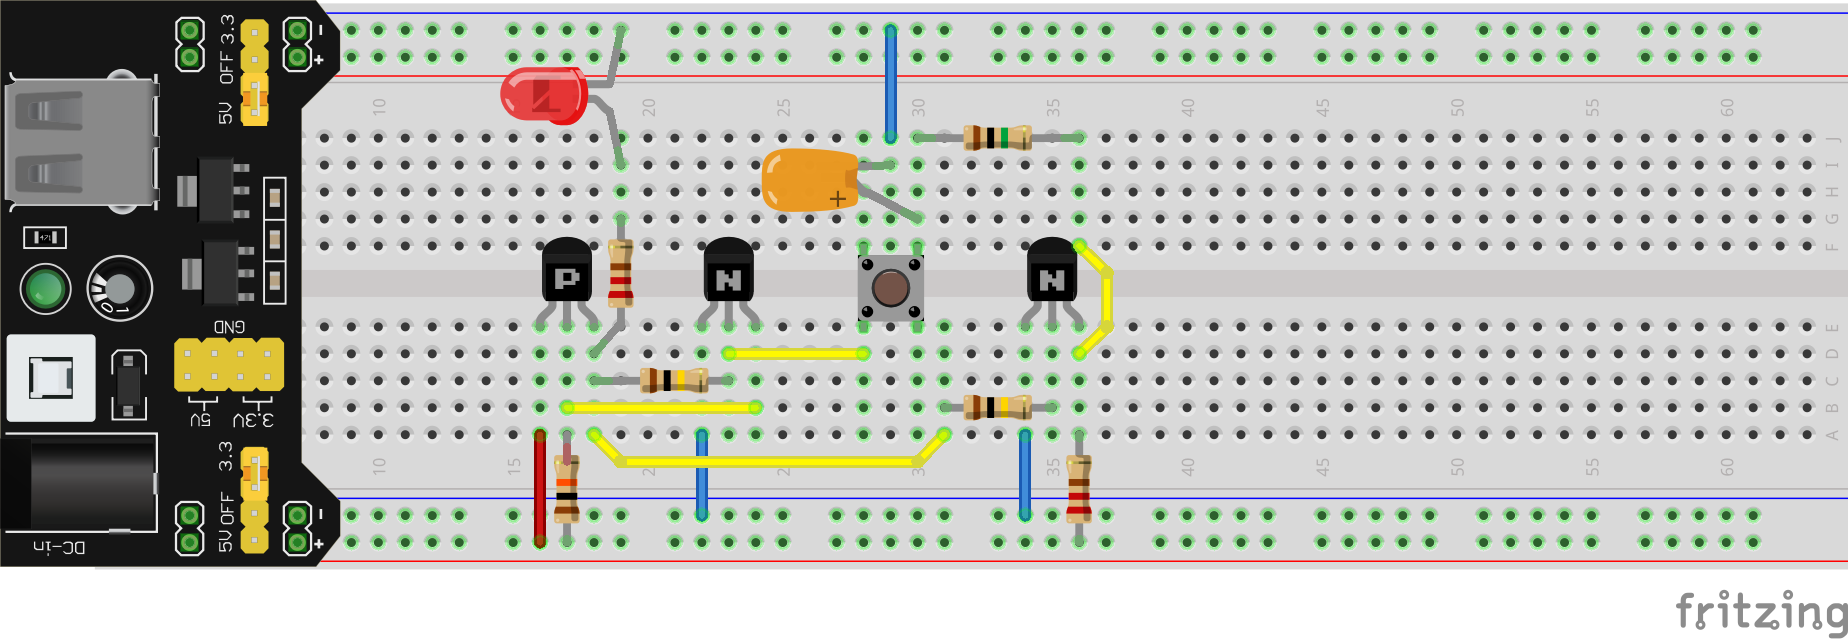
\includegraphics[width=\textwidth]{lesson_circuits/L8/lesson_8.png}
    \caption{Toggle Switch using BJTs Breadboard Schematic}
    \label{fig:toggle_bjt_sch}
\end{figure}
\begin{figure}[!htp]
    \centering
    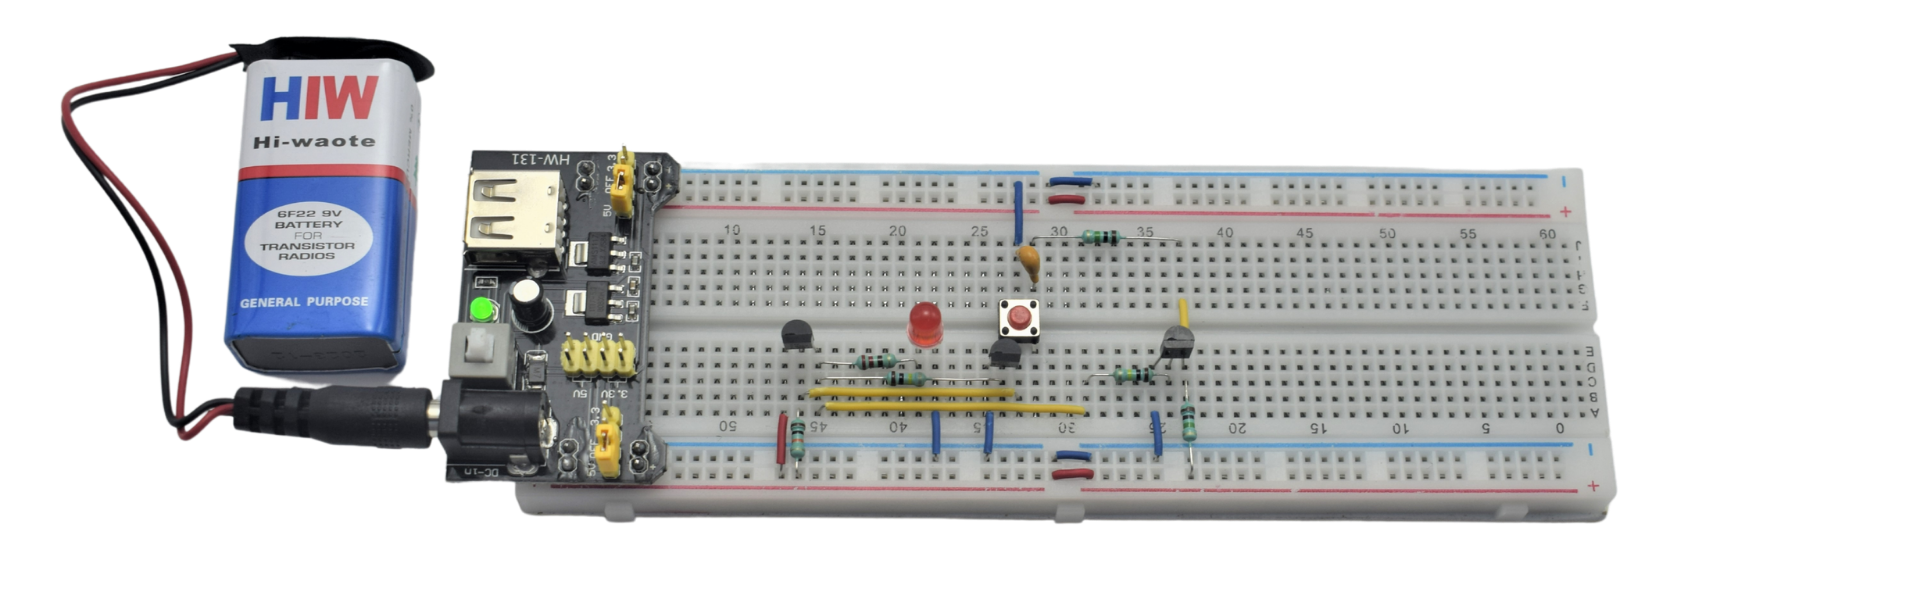
\includegraphics[width=\textwidth]{lesson_circuits/L8/L8-A.png}
    \caption{Toggle Switch: Off State}
    \label{fig:toggle_bjt_obb1}
\end{figure}
\begin{figure}[!htp]
    \centering
    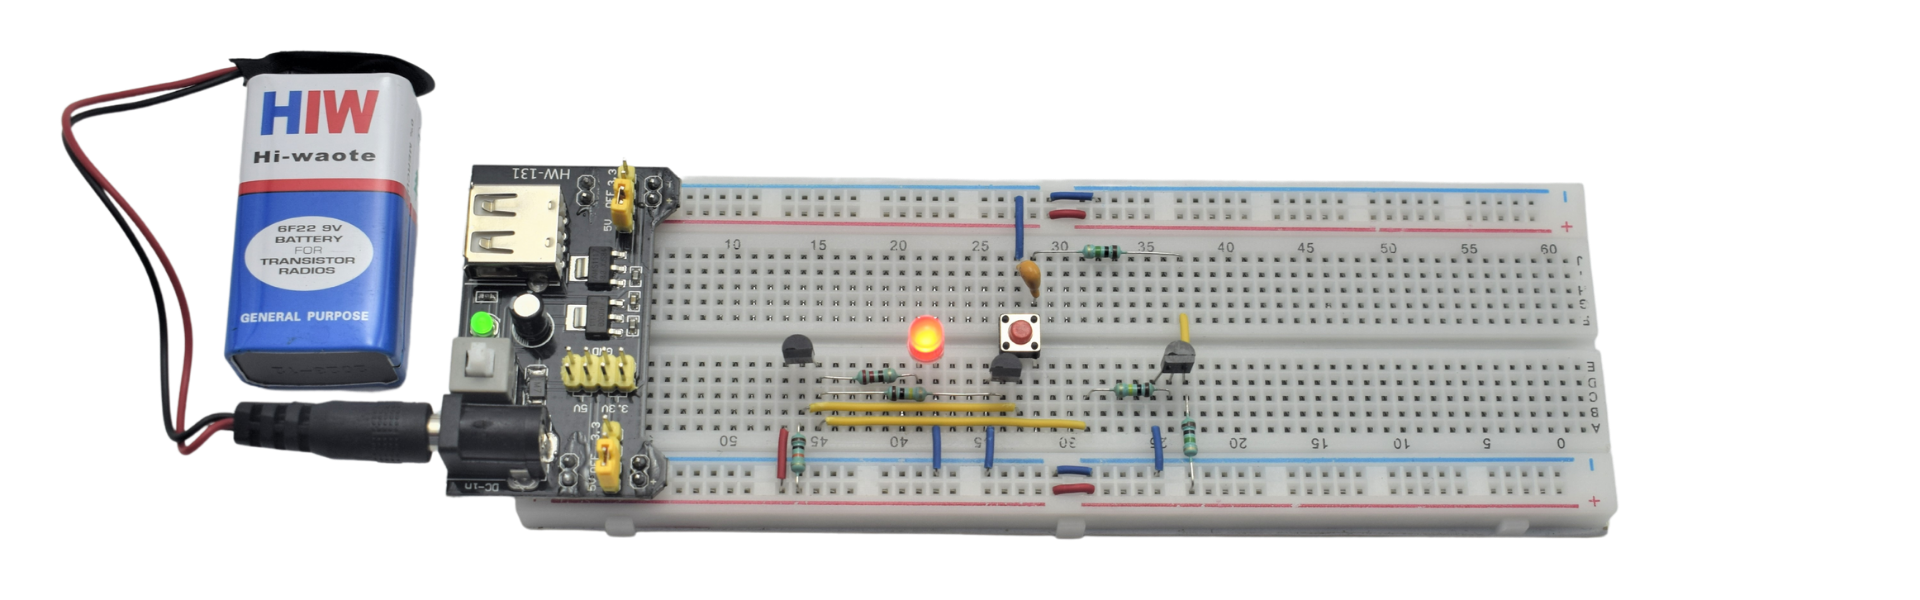
\includegraphics[width=\textwidth]{lesson_circuits/L8/L8-B.png}
    \caption{Toggle Switch: On State}
    \label{fig:toggle_bjt_obb2}
\end{figure}



\clearpage
\section{Lesson 9: Two Color LED Flasher using Transistors}
\subsection{Objective}
In this activity we will use the astable multivibrator to flash a rgb led.
\subsection{Components Required}
\begin{enumerate}
    \item Breadboard Power Supply $\times$ 1
    \item 9V Battery $\times$ 1
    \item 9V Battery Connector $\times$ 1
    \item Breadboard $\times$ 1
    \item RGB LED (Common Cathode) $\times$ 1
    \item \SI{220}{\ohm} $\times$ 2
    \item \SI{100}{\kilo\ohm} $\times$ 2
    \item 2N2222 NPN Transistor $\times$ 2
    \item \SI{10}{\micro\farad} $\times$ 2
    \item Male-Male jumper wire $\times$ 5
\end{enumerate}
\subsection{Circuit}
\begin{figure}[!htp]
    \centering
    \begin{circuitikz}[scale = 2]
        \draw (0,0) to[short, *-] (0,0) node[ground](gnd1){};
        \draw (0,0) to[full led, invert, color=green] (0,1);
        \draw (0,0) -- (0.5,0) to[full led, invert, color=red] (0.5,1);
        \draw (0,0) -- (-0.5,0) to[full led, invert, color=blue] (-0.5,1);
        \draw (-1.5,1.7) node[npn](t2){T2};
        \draw (1.5,1.7) node[npn, xscale=-1](t1){\scalebox{-1}[1]{T1}};
        \draw (t1.E) -| (0,1);
        \draw (t2.E) -| (-0.5,1);
        \draw (t1.C) to[short, -*] ++(0,0.5)
                to[R, l_=$\SI{220}{\ohm}$] ++(0,0.8)
                to[short, -*] ++(0,0.1) -- ++(1,0)
                to[R, l=$\SI{100}{\kilo\ohm}$] ++(0,-1)
                to[short, -*] ++(0,-0.2) |- (t1.B);
        \draw (t2.C) to[short, -*] ++(0,0.5)
                to[R, l=$\SI{220}{\ohm}$] ++(0,0.8)
                to[short, -*] ++(0,0.1) -- ++(-1,0)
                to[R, l_=$\SI{100}{\kilo\ohm}$] ++(0,-1)
                to[short, -*] ++(0,-0.4) |- (t2.B);
        \draw (-1.5, 3.48) to[short, -*] (0,3.48) node[vcc]{VCC}
                -- (1.5, 3.48);
        \draw ($(t2.C)+(0,0.5)$) to[C, l=$\SI{10}{\micro\farad}$] ++(1.3,0) 
                |- (2.5,2.28);
        \draw ($(t1.C)+(0,0.5)$) to[C, l_=$\SI{10}{\micro\farad}$] ++(-1.3,0) 
                |- (-2.5,2.08);
    \end{circuitikz}
    \caption{Two Color LED Flasher using Transistor}
    \label{fig:rgb_transistor}
\end{figure}
\subsection{Circuit Explanation}
This circuit operation is similar to that of astable multivibrator. Both the capacitors charge and discharge alternatively and thus turn on and off the transistors, causing the led to light up alternatively or in a flashing manner. By changing the capacitor and resistor values independently we can change the turn on and off time of both the LEDs.
\subsection{Circuit Picture}
\begin{figure}[!htp]
    \centering
    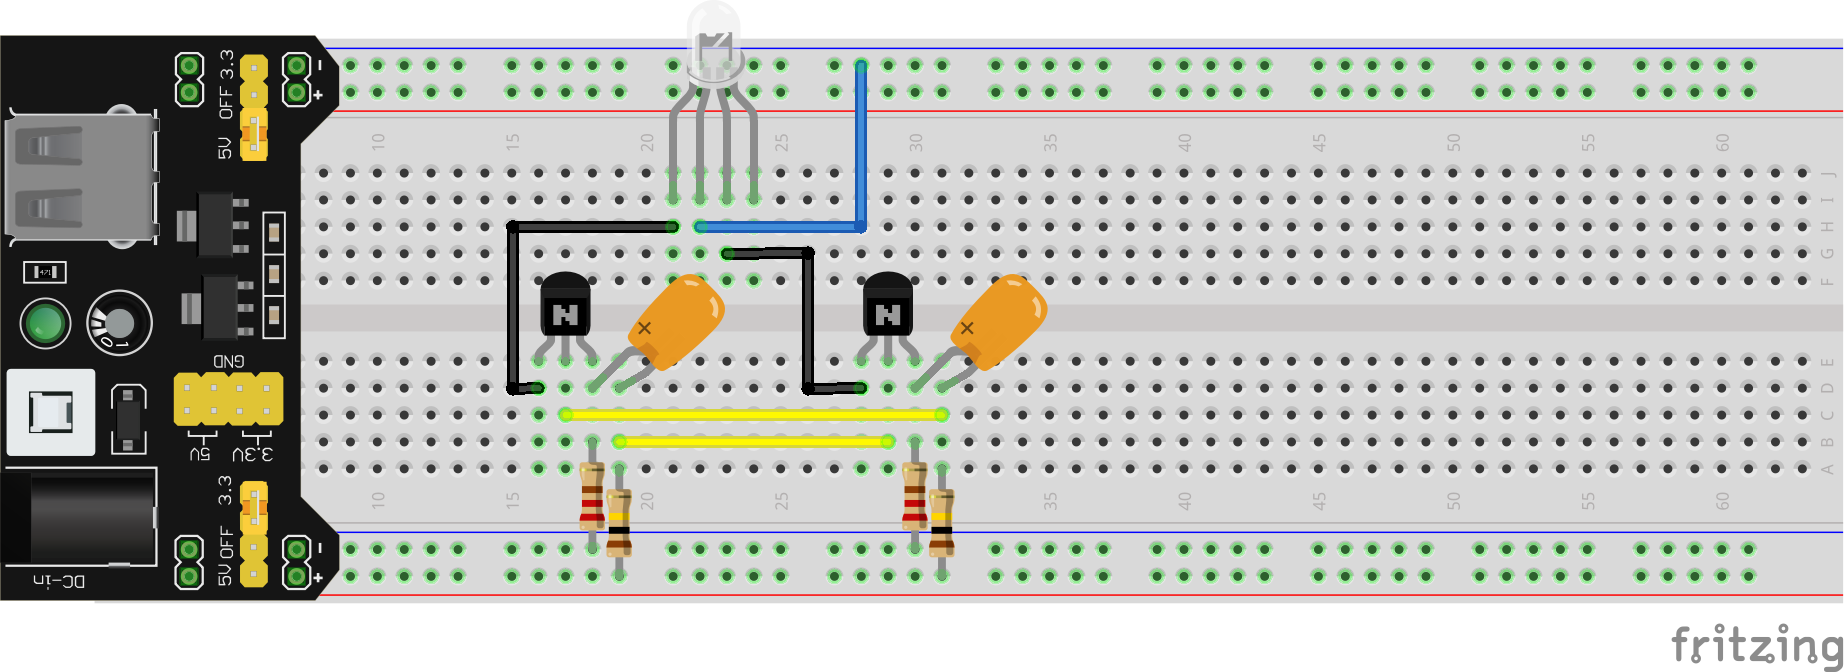
\includegraphics[width=\textwidth]{lesson_circuits/L9/lesson_9.png}
    \caption{Two Color LED flasher using BJTs Breadboard Schematic}
    \label{fig:two_led_bjt_sch}
\end{figure}
\begin{figure}[!htp]
    \centering
    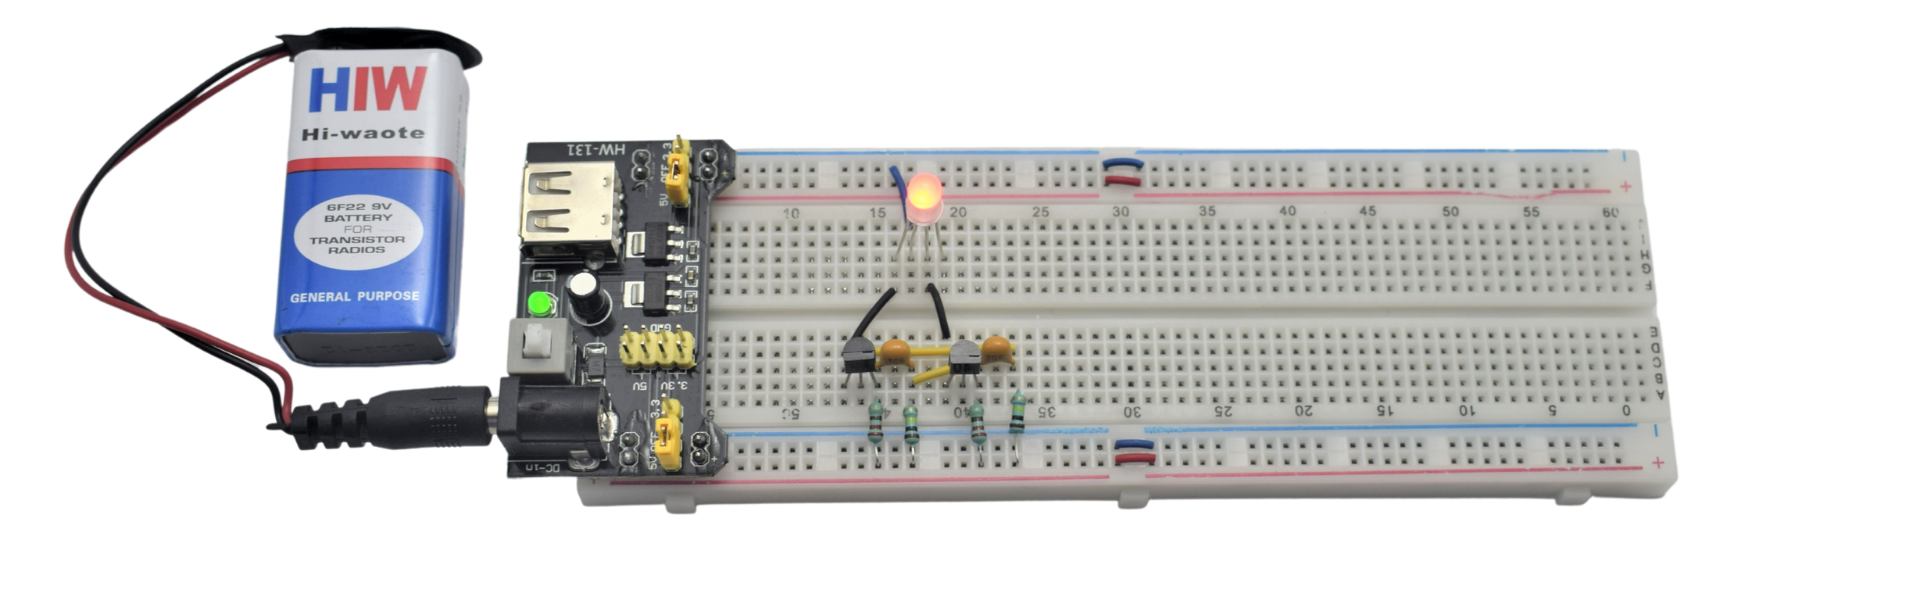
\includegraphics[width=\textwidth]{lesson_circuits/L9/L9-A.png}
    \caption{Two Color LED flasher}
    \label{fig:bjt_2led_obb}
\end{figure}



\clearpage
\section{Lesson 10: Light Sensitive LED using LDR}
\subsection{Objective}
In this activity we will make light sensitive LED, which will light up in darkness.
\subsection{Components Required}
\begin{enumerate}
    \item Breadboard Power Supply $\times$ 1
    \item 9V Battery $\times$ 1
    \item 9V Battery Connector $\times$ 1
    \item Breadboard $\times$ 1
    \item RGB LED (Common Cathode) $\times$ 1
    \item \SI{220}{\ohm} $\times$ 1
    \item \SI{100}{\kilo\ohm} $\times$ 1
    \item LDR (Photo-resistor) $\times$ 1
    \item Male-Male jumper wire $\times$ 3
\end{enumerate}
\subsection{Circuit}
\begin{figure}[!htp]
    \centering
    \begin{circuitikz}[scale = 2]
        \draw (0,0) node[ground](gnd1){};
        \draw (0,1) node[npn](t1){$T_1= 2N2222$};
        \draw (gnd1) -- ++(-1,0)
            to[sR,l=$LDR$] (-1,1)
            -- (t1.B);
        \draw (t1.C) to[empty led, invert, mirror] (0,2)
                to[R, l=$\SI{220}{\ohm}$] (0,3)
                node[vcc](vcc1){$V_cc$};
        \draw (vcc1) -| (-1,1) to[short, *-] ++(0,0);
        \draw (gnd1) -- (t1.E);
    \end{circuitikz}
    \caption{Light Sensitive LED}
    \label{fig:ldr_bjt_led}
\end{figure}
\subsection{Circuit Explanation}
We have used LDR in a voltage divider configuration. When there is change in light falling on the LDR, the voltage
drop across it will change due to change in it's resistance.
\begin{figure}[!htp]
    \centering
    \begin{circuitikz}[scale = 2]
        \draw (0,0) -- (-1,0)
            to[sR, l=$R_{LDR}$] (-1,1) node[](A){}
            to[R, l=$R_{fixed}$] (-1,2) -- (0,2);
        \draw[-latex]
            (A) to[short, *-] (0,1);
        \draw (-0.1,2.1) node[]{$V_{cc}$};
        \draw (-0.1,1.1) node[]{$V_{out}$};
        \draw (-0.1,0.1) node[]{$GND$};
    \end{circuitikz}
    \caption{LDR as Voltage Divider}
    \label{fig:ldr_volt_div}
\end{figure}

The output voltage ($V_{out}$) can be calculate by using the formula -
\begin{align*}
    V_{out} = V_{cc} \times \frac{R_{LDR}}{R_{LDR} + R_{fixed}}
\end{align*}
According to LDR data-sheet, we can find the threshold value of $R_{LDR}$ in dark and daylight, 
after that we need to find the value of $R_{fixed}$ such that the following conditions below are met -
\begin{enumerate}
    \item $0.7\si{\volt} \leq V_{out}$ in the dark.
    \item $0.7\si{\volt} > V_{out}$ in the daylight.
    \item The base current should be more than 20\si{\uA}
\end{enumerate}

In dark, $R_{LDR} = 550\si{\kohm}$ and in daylight, $R_{LDR} = 6\si{\kohm}$.

Let's work out each condition one by one.

\emph{The first condition}
\begin{align*}
    0.7\si{\V} & \leq V_{out} \\
    V_{out} & \leq V_{cc} \times \frac{R_{LDR}}{R_{LDR} + R_{fixed}} \\
    0.7\si{\V} & \leq 5\si{\V} \times \frac{550\si{\kohm}}{550\si{\kohm} +  R_{fixed}} \\
    R_{fixed} + 550\si{\kohm} & \leq \frac{5}{0.7} \times 550\si{kohm} \\
    R_{fixed} & \leq 3928.57\si{\kohm} - 550\si{\kohm} \\
    R_{fixed} & \leq 3.38\si{\Mohm} \\
\end{align*}

\emph{The second condition}
\begin{align*}
    0.7\si{\V} & > V_{out} \\
    V_{out} & > V_{cc} \times \frac{R_{LDR}}{R_{LDR} + R_{fixed}} \\
    0.7 & > 5\si{\V} \times \frac{6\si{\kohm}}{6\si{\kohm} + R_{fixed}} \\
    R_{fixed} + 6\si{\kohm} & > \frac{5}{0.7} \times 6\si{\kohm} \\
    R_{fixed} & > 42.86\si{\kohm} - 6\si{\kohm} \\
    R_{fixed} & > 36.86\si{\kohm} \\
\end{align*}

\emph{The third condition}
\begin{align*}
    V_{cc} & > 0.7\si{\V} + R_{fixed} \times I \\
    R_{fixed} & < \frac{5 - 0.7}{20\si{\uA}} \\
    R_{fixed} & < 215\si{\kohm} \\
\end{align*}

Now, analyzing all the above three conditions we see that - 
\begin{align*}
    36.86\si{\kohm} < R_{fixed} < 215\si{\kohm}
\end{align*}

We have selected $R_{fixed} = 100\si{\kohm}$.

\subsection{Circuit Picture}
\begin{figure}[!htp]
    \centering
    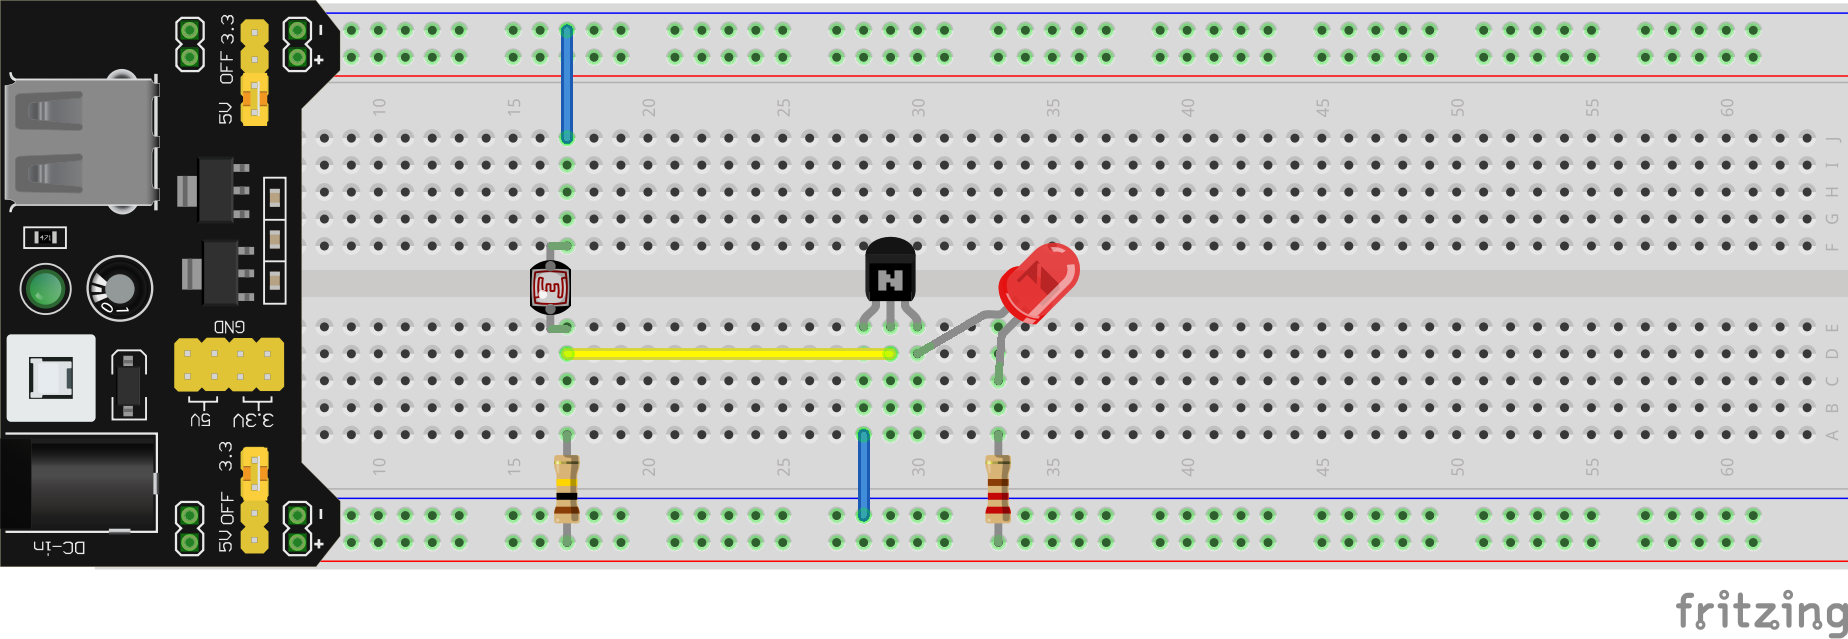
\includegraphics[width=\textwidth]{lesson_circuits/L10/lesson_10.png}
    \caption{Light sensitive LED Breadboard Schematic}
    \label{fig:light_sense_bjt_sch}
\end{figure}
\begin{figure}[!htp]
    \centering
    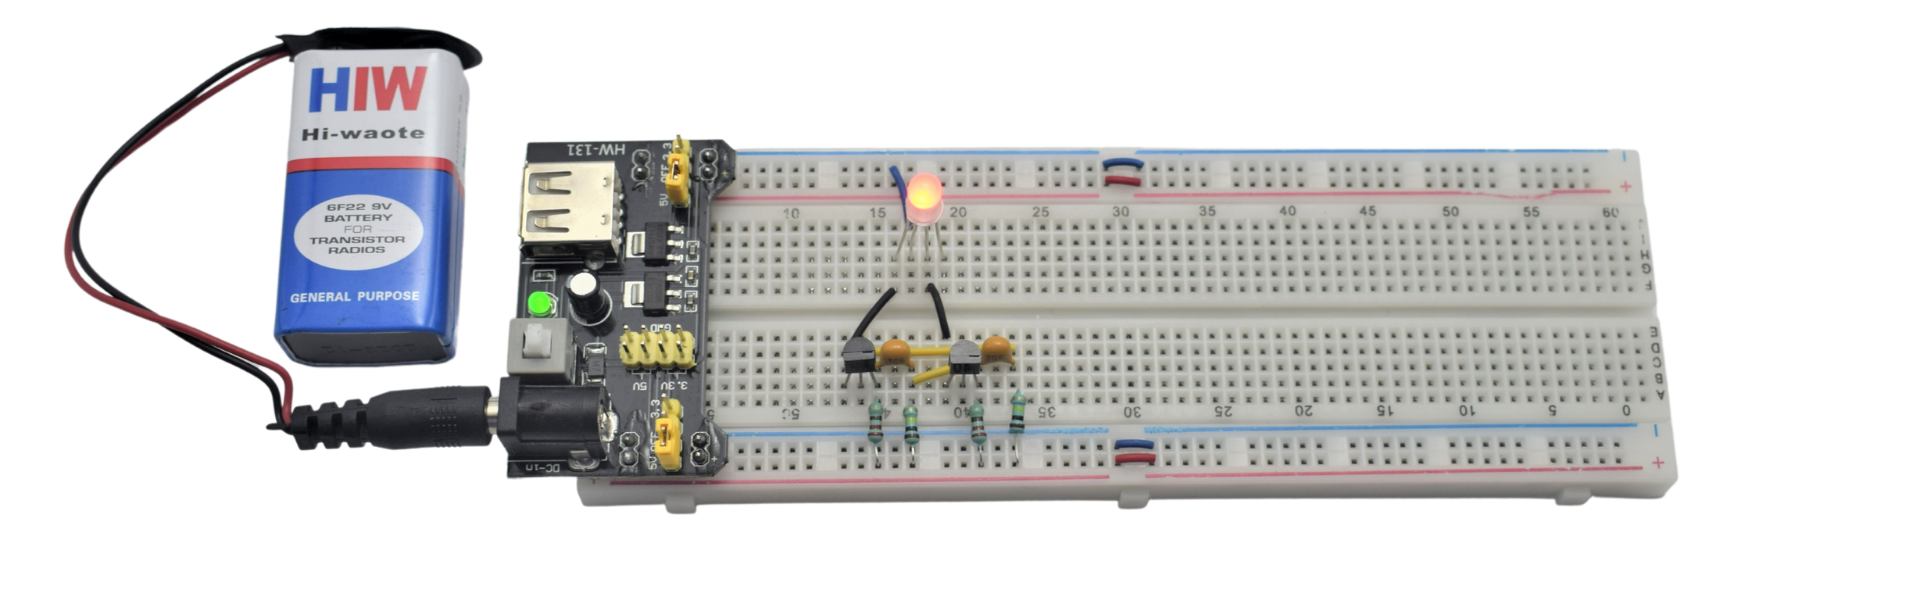
\includegraphics[width=\textwidth]{lesson_circuits/L9/L9-A.png}
    \caption{Light sensitive LED}
    \label{fig:ldr_bjt_working_obb}
\end{figure}